% !TEX program = xelatex
% =====================================================================
%  2026 高教社杯全国大学生数学建模竞赛  A 题  药材的烘干问题
%  电子版：\documentclass[withoutpreface,bwprint]{cumcmthesis}
%  纸质版：去掉 withoutpreface 选项再编译一次
%  编译：  xelatex 论文.tex  (两遍，生成交叉引用)
% =====================================================================
\documentclass[withoutpreface,bwprint]{cumcmthesis}
\usepackage{amsmath,amssymb}

\graphicspath{{../图表/}{./fig/}}
\captionsetup{font=small,labelfont=bf}
\newtheorem{proposition}{命题}
\newtheorem{remark}{注}

\lstset{
  basicstyle=\ttfamily\scriptsize,
  breaklines=true,
  columns=flexible,
  keepspaces=true,
  frame=single,
  framexleftmargin=2pt,
  xleftmargin=8pt,
  numbers=left,
  numberstyle=\tiny,
  numbersep=5pt,
  showstringspaces=false,
  commentstyle=\itshape,
  keywordstyle=\bfseries,
  extendedchars=true,
}

\title{中药材热风烘干过程的热湿耦合建模与坐标正则化谱方法求解}
\tihao{A}
\baominghao{}
\schoolname{}
\membera{}
\memberb{}
\memberc{}
\supervisor{}
\yearinput{2026}
\monthinput{9}
\dayinput{12}

\begin{document}
\maketitle

% =====================================================================
\begin{abstract}
\noindent
干燥是决定中药材成品品质的关键工序。针对圆柱形药材的热风烘干过程，本文建立了
温度--水分浓度耦合的轴对称扩散模型，并提出以\textbf{坐标正则化}为核心的谱方法求解方案。

\textbf{模型建立}：由壳层守恒推得 $\rho c_p\partial_tT=r^{-1}\partial_r(rk\partial_rT)$ 与
$\partial_tC=r^{-1}\partial_r(rD\partial_rC)$，表面取 Robin 条件；由长径比
$L/R_0=12.5$（轴向与径向特征时间之比 $(L/R_0)^2=156$）论证一维轴对称简化合理。
烘房环境由附件 1 实测序列标定为一阶惯性式，用 Levenberg--Marquardt 二参数拟合
（初值固定为实测值）得 $T_{\rm set}=50.212\,^\circ$C、$\tau_T=1877.5$ s
（RMSE $0.336\,^\circ$C，$R^2=0.9957$）与 $C_{\rm set}=0.050908$ kg/kg、
$\tau_C=2776.3$ s（RMSE $8.1\times10^{-4}$，$R^2=0.9901$），残差经正态性与自相关诊断。
问题 4 在物质坐标下严格推导，证明各向同性收缩时对流项为零。

\textbf{方法创新}：取 $u=\xi^2=(r/R)^2$ 为自变量，圆柱 Laplace 算子化为
$r^{-1}\partial_r(rD\partial_r)=(4/R^2)\partial_u(uD\partial_u)$，在轴心处\textbf{完全正则}，
从而免去常规离散所必需的最内控制体特殊处理；解在 $u$ 上解析，故可用
Chebyshev--Gauss--Lobatto 谱配置获得谱精度，实测 $N=8$ 即达 $10^{-10}$。
时间方向采用变阶变步长隐式 BDF，物性每步重估。问题 1 因常物性下两场解耦、
环境为指数型，用准静态分解导出 \textbf{Bessel--Duhamel 闭式级数解}，2 项即达机器精度。

\textbf{主要结果}：问题 1 在 $t=1800$ s 时中心温度 $34.0425\,^\circ$C、表面 $37.1989\,^\circ$C、
表面含水 $1.5109$ kg/kg；问题 2 在 $t=3$ h 时中心温度 $49.9051\,^\circ$C、
中心含水 $1.7673$、表面含水 $1.0083$ kg/kg；问题 3 得
$t_{\rm dry}=205575.5$ s $=57.1043$ h；问题 4 计入收缩后
$t_{\rm dry}=182778.3$ s $=50.7717$ h，收缩使扩散长度平方降至
$(R/R_0)^2=0.359$，烘干时间缩短 $11.1\%$。

\textbf{模型检验}：用三条相互独立的路线互证——闭式解析解、谱配置法、
两族不同离散的有限体积格式，互差不超过 $2\times10^{-6}$；谱解与对照格式在连续极限上
吻合到 $3\times10^{-8}$；另给出残差正态性（直方图与 Q-Q 图）、时间积分器稳定性
（四种配置极差 $0.007$ s）与空间收敛阶。进一步分析表明\textbf{烘干时长是全题最敏感的量}：
判据附近 $\mathrm{d}C_0/\mathrm{d}t\approx-2.9\times10^{-7}$ s$^{-1}$，
$1$ s 仅对应 $2.9\times10^{-7}$ kg/kg；定步长冻结系数的 $\theta$ 法在时间上只有
\textbf{一阶}精度，长时间段放宽步长会使 $t_{\rm dry}$ 被低估约 $15$ s。

\textbf{灵敏度分析}（真实运行，12 组扰动）：活化温度 $E=3850$ K 主导不确定性，
$\pm2\%$ 使 $t_{\rm dry}$ 变化 $+23.9\%/-18.6\%$；活化浓度指数 $a$ 次之（$\pm2\%$ 约 $\pm4.8\%$）；
而 $D_0$、$T_{\rm set}$、$h_m$ 影响均在 $2\%$ 以内，$h$ 的影响小于 $0.01\%$。
这说明应优先提高 $E$ 与 $a$ 的标定精度。

\keywords{热湿耦合扩散；Robin 边界；坐标正则化；Chebyshev 谱配置；自适应隐式积分；
Bessel--Duhamel 展开；物质坐标；烘干时长收敛性}
\end{abstract}

% =====================================================================
\section{问题重述}

\subsection{问题背景}

干燥是中药材产地加工与炮制过程中的关键工序，直接决定成品的有效成分保留率、
外观等级与贮藏稳定性。热风烘干因设备简单、成本低而应用最广。该过程分为两个阶段：
先经历\textbf{预热平衡阶段}，药材由环境温度被加热到接近烘房温度、内部建立稳定的温度梯度；
随后进入\textbf{恒温干燥阶段}，在近似恒定的温湿度环境下水分由内部迁至表面并被气流带走。
工艺参数选择不当会导致干燥过慢（能耗高、周期长）、表面「结壳」（外干内湿）
或温度过高（破坏热敏性成分）。传统的「试错--检测」优化模式周期长、成本高，
因此有必要用数理模型刻画药材内部温度与水分浓度的时空演化，以预测干燥时长、指导工艺设计。

\subsection{题目条件}

某中药材形状近似为圆柱：长 $L=25$ cm、半径 $R_0=2$ cm。烘干开始时药材温度
$T_0=28\,^\circ$C，水分浓度（干基含水率）$C_0=2.55$ kg/kg。
烘房温度与水分浓度随时间的变化由附件 1 给出（$0\sim14400$ s，每 $60$ s 一点，共 $241$ 点）；
干燥过程中药材半径变化由附件 2 给出（$0\sim259200$ s，每 $1800$ s 一点，共 $145$ 点）。
附录 2--4 分别给出问题 1、问题 2--3、问题 4 所需的物性经验关系。

\subsection{需要解决的问题与量化子任务}

\begin{longtable}{@{}p{1.5cm}p{4.6cm}p{4.4cm}p{4.6cm}@{}}
\toprule
问题 & 输入 & 输出 & 判定标准 \\
\midrule
\endfirsthead
\toprule
问题 & 输入 & 输出 & 判定标准 \\
\midrule
\endhead
一 & 附录 2 物性、附件 1 环境、初值 $(28\,^\circ{\rm C},2.55)$ &
$t=100\sim1800$ s、$r=0\sim2$ cm 的温度与含水率；$1800$ s 内每 $1$ s、每 $0.1$ cm 全结果 &
表 1、表 2 保留 4 位小数；\texttt{result1.xlsx} \\
二 & 附录 3 变物性、两阶段工艺 & $3$ h 内每 $0.5$ h 的温度与含水率；全结果 &
表 3、表 4；\texttt{result2.xlsx} \\
三 & 同问题二，时间跨度至干燥结束 & 烘干时长；每 $6$ h、每 $0.5$ cm 的含水率 &
\textbf{处处} $C<0.15$ kg/kg；表 5；\texttt{result3.xlsx} \\
四 & 附录 4 物性、附件 2 的 $R(t)$ & 烘干时长；每 $6$ h、每 $0.5$ cm 的含水率 &
同问题三；表 6；\texttt{result4.xlsx} \\
\bottomrule
\end{longtable}

\subsection{数据探索}

如图~\ref{fig:env} 所示，附件 1 的两个序列均呈明显一阶惯性上升形态：
温度由 $28\,^\circ$C 升至约 $50.2\,^\circ$C 后稳定，含湿量由 $0.01963$ kg/kg
升至约 $0.0509$ kg/kg 后稳定，在 $t\approx4$ h 处进入平台——
这一形态直接决定了后续的环境建模方式（一阶惯性式）与工艺分段（$t=14400$ s）。
附件 2 的半径序列（图~\ref{fig:radius}）单调不增，由 $R(0)=2.000$ cm 迅速下降，
至 $t>207000$ s 后稳定在 $R\approx1.198\sim1.200$ cm（$R/R_0=0.599$），
$90\%$ 的收缩在前 $10$ h 内完成，$|\mathrm{d}R/\mathrm{d}t|$ 在 $t=0$ 处最大。

\begin{figure}[H]
\centering
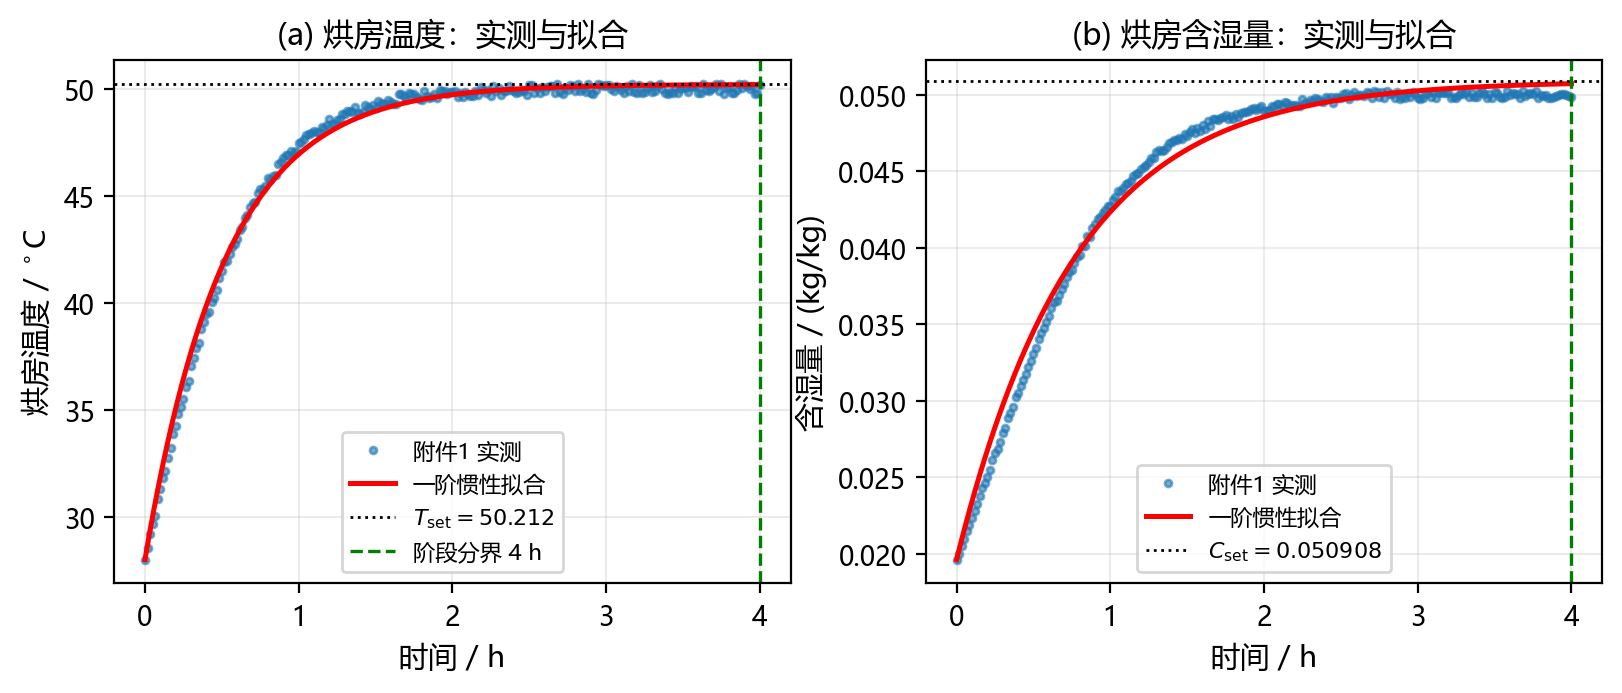
\includegraphics[width=\textwidth]{fig01_env_fit.png}
\caption{附件 1 烘房温度与含湿量的实测序列及一阶惯性拟合}
\label{fig:env}
\end{figure}

\begin{figure}[H]
\centering
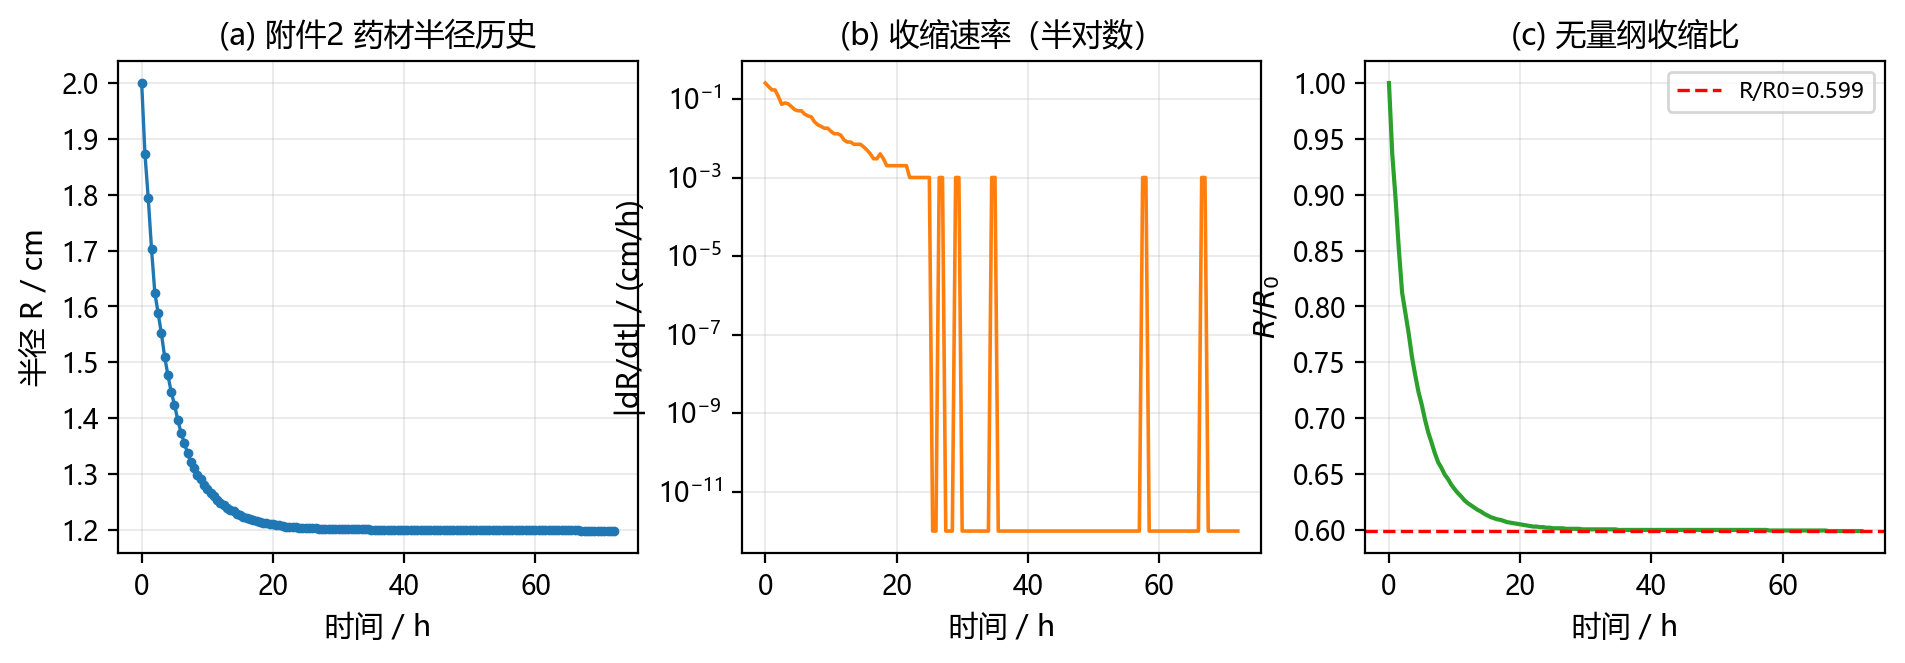
\includegraphics[width=\textwidth]{fig04_radius.png}
\caption{附件 2 药材半径历史、收缩速率与无量纲收缩比}
\label{fig:radius}
\end{figure}

% =====================================================================
\section{问题分析}

\subsection{总体思路与建模理由链}

本题的核心是一个\textbf{变物性、非线性、带 Robin 边界、且（问题 4 中）求解域随时间收缩}
的轴对称扩散问题。四个问题共用同一套控制方程，差别只在物性关系、环境口径与几何是否收缩。
因此采取「\textbf{一套方程、一套求解框架、四组参数}」的总体思路，把工作量集中在
「把模型建准」与「把数值解算到可信」两件事上。技术路线如图~\ref{fig:flow} 所示。

\begin{figure}[H]
\centering
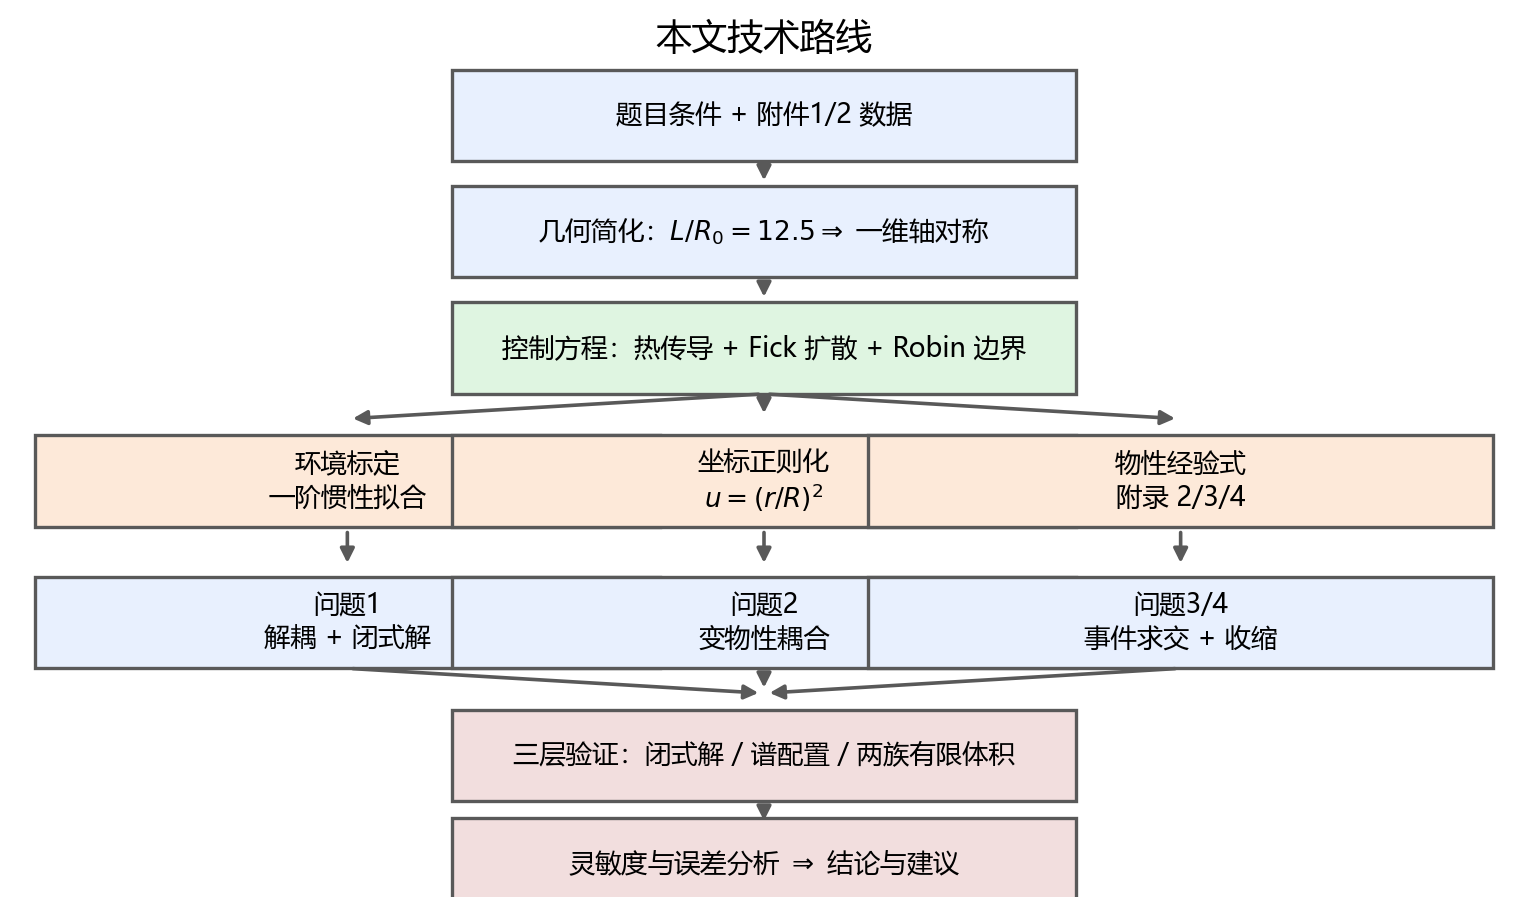
\includegraphics[width=0.92\textwidth]{fig25_flow.png}
\caption{本文技术路线图}
\label{fig:flow}
\end{figure}

\textbf{理由链（以问题 1 为例）}：\emph{机理}——热风对流的边界驱动 + 内部导热/扩散；
\emph{模型形式}——圆柱坐标下的抛物型耦合方程组 + Robin 边界；
\emph{可辨识参数}——$\rho,c_p,k,h,h_m$ 由附录 2 给出，$D(C)$ 由附录 2 的经验式给出，
环境由附件 1 标定，均不含不可辨识参数；
\emph{求解方法}——温度场与水分场解耦 $\Rightarrow$ 温度场可闭式求解，水分场用谱配置；
\emph{可验证性}——温度场有闭式解作绝对基准，水分场可用两族离散互证。

\subsection{各问关键点}

\begin{itemize}[leftmargin=1.7em,itemsep=2pt]
\item \textbf{问题 1}：关键在于识别「两场解耦」。附录 2 给的是常数物性、$D$ 只依赖 $C$，
温度方程与水分方程可独立求解；又因烘房温度恰为指数型，温度场可用准静态分解化为闭式级数解。
物理预期为「热快质慢」：$\mathrm{Fo}_T(1800\,{\rm s})=0.760$ 而 $\mathrm{Fo}_D=0.0222$。
\item \textbf{问题 2}：关键是两阶段工艺刻画与变物性耦合。附录 3 的 $D$ 同时依赖 $C$ 与 $T$，
两场真正耦合；温度 $2$ h 内基本平衡，此后药材近似等温体，水分剖面由平缓转为陡峭。
\item \textbf{问题 3}：关键是判据的数学表述与极值点位置。判据是逐点的「处处低于」，
而非平均值；由圆柱几何对称性，中心扩散路径最长，必然是最后干燥点。本文不预设这一点，
而逐时刻对全场节点取最大。
\item \textbf{问题 4}：关键是移动边界。各向同性收缩下若在固定 $r$ 坐标直接套用扩散方程
会漏掉一个对流项，必须改用物质坐标；同时表格列名是「当前物理距离」，
与求解坐标不是一回事，采样须逐时刻换算。
\end{itemize}

% =====================================================================
\section{模型假设}

\begin{enumerate}[leftmargin=1.9em,itemsep=2pt]
\item \textbf{轴对称一维简化}。药材为无限长圆柱，温度与水分只依赖 $r$ 和 $t$。
\emph{成立条件}：长径比 $L/R_0=12.5$，轴向与径向特征时间之比 $(L/R_0)^2=156$；
且轴向送风均匀、端面对流条件对称。
\item \textbf{局部热平衡}。骨架与内部水分在同一位置瞬时达到热平衡，用单一温度描述。
\emph{成立条件}：$\mathrm{Le}=D/\alpha=2.9\times10^{-2}\ll1$，热扩散远快于水分扩散。
\item \textbf{干物质不迁移}。干燥中水分迁移，干物质骨架只随整体收缩运动。
这是干基含水率的定义方式，也是问题 4 物质坐标推导的前提。
\item \textbf{表面传热传质为对流型}。由 $h$ 与 $h_m$ 控制，且过程中保持常数。
\emph{依据}：题目直接给定 $h=25$ W/(m$^2\cdot$K)、$h_m=8\times10^{-7}$ m/s。
\item \textbf{物性经验关系适用}。三组物性式在其适用区间内成立。因题目未给出标定区间，
本文在 \S\ref{sec:sens} 中对 $E$ 与 $a$ 做 $\pm2\%$ 扰动评估外推风险。
\item \textbf{烘房环境可分段描述}。$0\sim14400$ s 按一阶惯性式变化，其后恒定
（烘房持续排湿）。\emph{依据}：附件 1 在 $t\approx4$ h 达到设定值并稳定。
\item \textbf{收缩各向同性}。同一物质点在任意时刻满足 $r(t)=\xi R(t)$。
\emph{依据}：题目只给出半径方向的收缩数据；\S\ref{sec:shrink} 证明该假设下物质坐标
对流项严格为零。
\item \textbf{不计蒸发潜热引起的表面热流}。基准模型只保留显热项。
\emph{依据}：题目未提供汽化潜热与孔隙率等标定数据，该项无法由题面数据定量，
本文在 \S\ref{sec:eval} 列为模型局限。
\end{enumerate}

% =====================================================================
\section{符号说明}

\begin{center}
\small
\begin{longtable}{@{}p{2.5cm}p{8.4cm}p{3.5cm}@{}}
\toprule
符号 & 含义 & 单位 \\
\midrule
\endfirsthead
\toprule
符号 & 含义 & 单位 \\
\midrule
\endhead
$r$ & 到药材中心的物理距离 & m \\
$R(t)$ & 当前半径（问题 4 变化，其余恒为 $R_0$） & m \\
$R_0,\ L$ & 初始半径、药材长度 & m \\
$T(r,t)$ & 药材温度 & $^\circ$C \\
$C(r,t)$ & 水分浓度（干基含水率） & kg/kg \\
$T_{\rm air},C_{\rm air}$ & 烘房温度、含湿量 & $^\circ$C, kg/kg \\
$\rho,\ c_p,\ k$ & 密度、比热容、导热系数 & kg/m$^3$, J/(kg$\cdot$K), W/(m$\cdot$K) \\
$D$ & 水分浓度扩散系数 & m$^2$/s \\
$h,\ h_m$ & 对流换热系数、对流传质系数 & W/(m$^2$K), m/s \\
$\alpha$ & 热扩散率 $k/(\rho c_p)$ & m$^2$/s \\
$\mathrm{Bi},\mathrm{Bi}_m$ & 热/传质 Biot 数 & --- \\
$\mathrm{Fo},\mathrm{Fo}_D$ & 热/传质 Fourier 数 & --- \\
$\mathrm{Le}$ & Lewis 数 $D/\alpha$ & --- \\
$\xi$ & 物质坐标 $r/R(t)$ & --- \\
$u$ & 正则化坐标 $\xi^2$ & --- \\
$E$ & Arrhenius 活化温度（$3850$ K） & K \\
$a$ & 活化浓度指数 & kg/kg \\
$t_{\rm dry}$ & 烘干时长（处处 $C<0.15$ 的首达时刻） & s \\
\bottomrule
\end{longtable}
\end{center}

% =====================================================================
\section{模型的建立}

\subsection{几何简化}

药材为半径 $R_0=2$ cm、长 $L=25$ cm 的圆柱。轴向导热特征时间
$L^2/\alpha\approx3.70\times10^5$ s（约 $4.3$ 天），径向 $R_0^2/\alpha\approx2369$ s，
两者之比恰为 $(L/R_0)^2=156$，相差约 $2.2$ 个数量级；同时烘房气流沿轴向均匀送风。
故端面效应与轴向梯度可以忽略，问题化为轴对称一维径向问题。

\subsection{传热控制方程}

在半径 $r$ 处取厚度 $\mathrm{d}r$、长 $L$ 的环形壳层，壳层内能的时变率等于净导入的导热热流：
\begin{equation}
\rho c_p(2\pi rL\,\mathrm{d}r)\frac{\partial T}{\partial t}
=-\big[q_r\cdot2\pi rL\big]_r^{r+\mathrm{d}r},\qquad q_r=-k\frac{\partial T}{\partial r},
\end{equation}
整理得
\begin{equation}
\rho(C)c_p(C)\frac{\partial T}{\partial t}
=\frac{1}{r}\frac{\partial}{\partial r}\left(rk(C)\frac{\partial T}{\partial r}\right).
\label{eq:energy}
\end{equation}

\subsection{传质控制方程}

以干基浓度 $C$ 为变量，水分通量 $j_r=-\rho_dD\partial_rC$，
其中 $\rho_d=\rho/(1+C)$ 为单位湿体积内的干物质质量。
壳层内干物质质量 $2\pi rL\rho_d\mathrm{d}r$ 不随时间变化，故控制体随干物质一起运动：
\begin{equation}
\frac{\partial C}{\partial t}
=\frac{1}{r}\frac{\partial}{\partial r}\left(rD(C,T)\frac{\partial C}{\partial r}\right).
\label{eq:mass}
\end{equation}

\subsection{边界条件与初始条件}

中心对称：$\partial_rT(0,t)=\partial_rC(0,t)=0$。
表面 Robin 条件（$r=R$）：
\begin{equation}
-k\left.\frac{\partial T}{\partial r}\right|_{r=R}=h(T_s-T_{\rm air}(t)),
\qquad
-D\left.\frac{\partial C}{\partial r}\right|_{r=R}=h_m(C_s-C_{\rm air}(t)),
\label{eq:robin}
\end{equation}
其中 $T_s=T(R,t)$、$C_s=C(R,t)$。初始条件：
$T(r,0)=28\,^\circ$C，$C(r,0)=2.55$ kg/kg。

\subsection{烘房环境数据的标定}
\label{sec:calib}

附件 1 是带噪实测序列，直接作边界会把测量噪声注入解。由图~\ref{fig:env} 的一阶惯性形态，
先作一阶惯性拟合，\textbf{初值固定为实测初值}：
\begin{equation}
T_{\rm air}(t)=T_{\rm set}-(T_{\rm set}-28)e^{-t/\tau_T},
\qquad
C_{\rm air}(t)=C_{\rm set}-(C_{\rm set}-0.01963)e^{-t/\tau_C}.
\label{eq:ambient}
\end{equation}
用 Levenberg--Marquardt 非线性最小二乘（初值固定，每式只有 $2$ 个自由参数）得

\begin{table}[H]
\centering
\small
\caption{烘房环境一阶惯性标定结果}
\begin{tabular}{@{}lcccc@{}}
\toprule
参数 & 拟合值 & 标准误 & RMSE & $R^2$ \\
\midrule
$T_{\rm set}$ / $^\circ$C & 50.2121 & 0.0303 & \multirow{2}{*}{0.336 $^\circ$C} & \multirow{2}{*}{0.9957} \\
$\tau_T$ / s & 1877.49 & 12.74 & & \\
$C_{\rm set}$ / (kg/kg) & 0.050908 & $9.3\times10^{-5}$ & \multirow{2}{*}{$8.1\times10^{-4}$} & \multirow{2}{*}{0.9901} \\
$\tau_C$ / s & 2776.34 & 31.71 & & \\
\bottomrule
\end{tabular}
\end{table}

计算中把标定参数按其有效位数取用（$T_{\rm set}=50.212$、$\tau_T=1877.5$、$\tau_C=2776.3$）。
该取舍在 $T(R,1800\,{\rm s})$ 上仅造成约 $6\times10^{-5}\,^\circ$C 的变化，
比标定标准误小三个数量级。

工艺分段：由附件 1 可见烘房在 $t\approx4$ h 达到设定值并稳定，故取
\begin{equation}
(T_{\rm air},C_{\rm air})=
\begin{cases}
\text{式}\eqref{eq:ambient}, & 0\le t\le14400\ {\rm s},\\[2pt]
(50.212\,^\circ{\rm C},\ 0.050908\ {\rm kg/kg}), & t>14400\ {\rm s}.
\end{cases}
\label{eq:stage}
\end{equation}

\subsection{物性经验关系与量纲检查}

\begin{table}[H]
\centering
\small
\caption{三组物性经验关系（附录 2--4）}
\begin{tabular}{@{}lccc@{}}
\toprule
 & 问题 1（附录 2） & 问题 2、3（附录 3） & 问题 4（附录 4） \\
\midrule
$\rho$ / (kg/m$^3$) & $820$ & $650+128C$ & $760+90C$ \\
$c_p$ / (J/(kg$\cdot$K)) & $2600$ & $1450+2736\dfrac{C}{C+1}$ & $1850+2150\dfrac{C}{C+1}$ \\
$k$ / (W/(m$\cdot$K)) & $0.36$ & $0.21+0.38\dfrac{C}{C+1}$ & $0.12+0.20\dfrac{C}{C+1}$ \\
$D$ / (m$^2$/s) & $7\times10^{-9}e^{-0.89/C}$ &
$2.4\times10^{-3}e^{-0.45/C}e^{-3850/T}$ &
$4.2\times10^{-4}e^{-0.30/C}e^{-3850/T}$ \\
\bottomrule
\end{tabular}
\end{table}

$e^{-3850/T}$ 为 Arrhenius 因子，对应活化能 $E_a=3850R_g=32.0$ kJ/mol。
量纲检查：$3850$ K 量纲为温度，$T$ 须取绝对温度；
$a$ 与 $C$ 同量纲（kg/kg），故 $a/C$ 无量纲。

\begin{remark}[经验式的读法自检]
附录 2 写成 $D=7\times10^{-9}e^{-0.89/C}$，指数部分有两种读法。
若读作 $e^{-0.89C}$，则 $C$ 由 $2.55$ 降到 $0.15$ 时 $D$ 反而\textbf{增大} $8.5$ 倍
（$e^{-0.89\times0.15}/e^{-0.89\times2.55}=8.47$），与「越干越难扩散」的降速干燥事实矛盾；
读作 $e^{-0.89/C}$ 时 $D$ 下降 $266$ 倍，正是降速干燥所要求的。
附录 3 同判：$e^{-0.45/C}$ 使 $D$ 由 $C=2.55$ 到 $C=0.15$ 下降 $16.8$ 倍。
故三个 $D$ 式中的指数一律读作 $e^{-a/C}$。

温度取绝对温度：由附录 3 在 $C=2.55$、$T=50\,^\circ$C 处得
$D=1.347\times10^{-8}$ m$^2$/s，量级与生物质材料有效水分扩散系数的常见范围
（$10^{-10}\sim10^{-8}$ m$^2$/s，见文献~[14]）相符；
若把 $T$ 误按摄氏度代入，$e^{-3850/50}\approx0$，$D$ 退化为零，显然不合理。
\end{remark}

\subsection{无量纲分析}

定义 $\mathrm{Bi}=hR_0/k$、$\mathrm{Bi}_m=h_mR_0/D$、
$\mathrm{Fo}=\alpha t/R_0^2$、$\mathrm{Le}=D/\alpha$。取问题 1 参数：
$\alpha=1.6886\times10^{-7}$ m$^2$/s，$\mathrm{Bi}=1.3889$，
$D(C_0)=4.9377\times10^{-9}$ m$^2$/s，$\mathrm{Bi}_m=3.2404$，$\mathrm{Le}=2.9\times10^{-2}$，
于是 $\mathrm{Fo}_T(1800\,{\rm s})=0.760$、$\mathrm{Fo}_D(1800\,{\rm s})=0.0222$
（图~\ref{fig:dimless}）。两条先验结论：其一 $\mathrm{Fo}_D\ll\mathrm{Fo}_T$，
温度先于水分达到准平衡；其二 $\mathrm{Bi}_m$ 量级为 $1$，
内部扩散阻力与外部对流传质阻力相当，必须保留 Robin 条件而不能把表面当作平衡边界。

\begin{figure}[H]
\centering
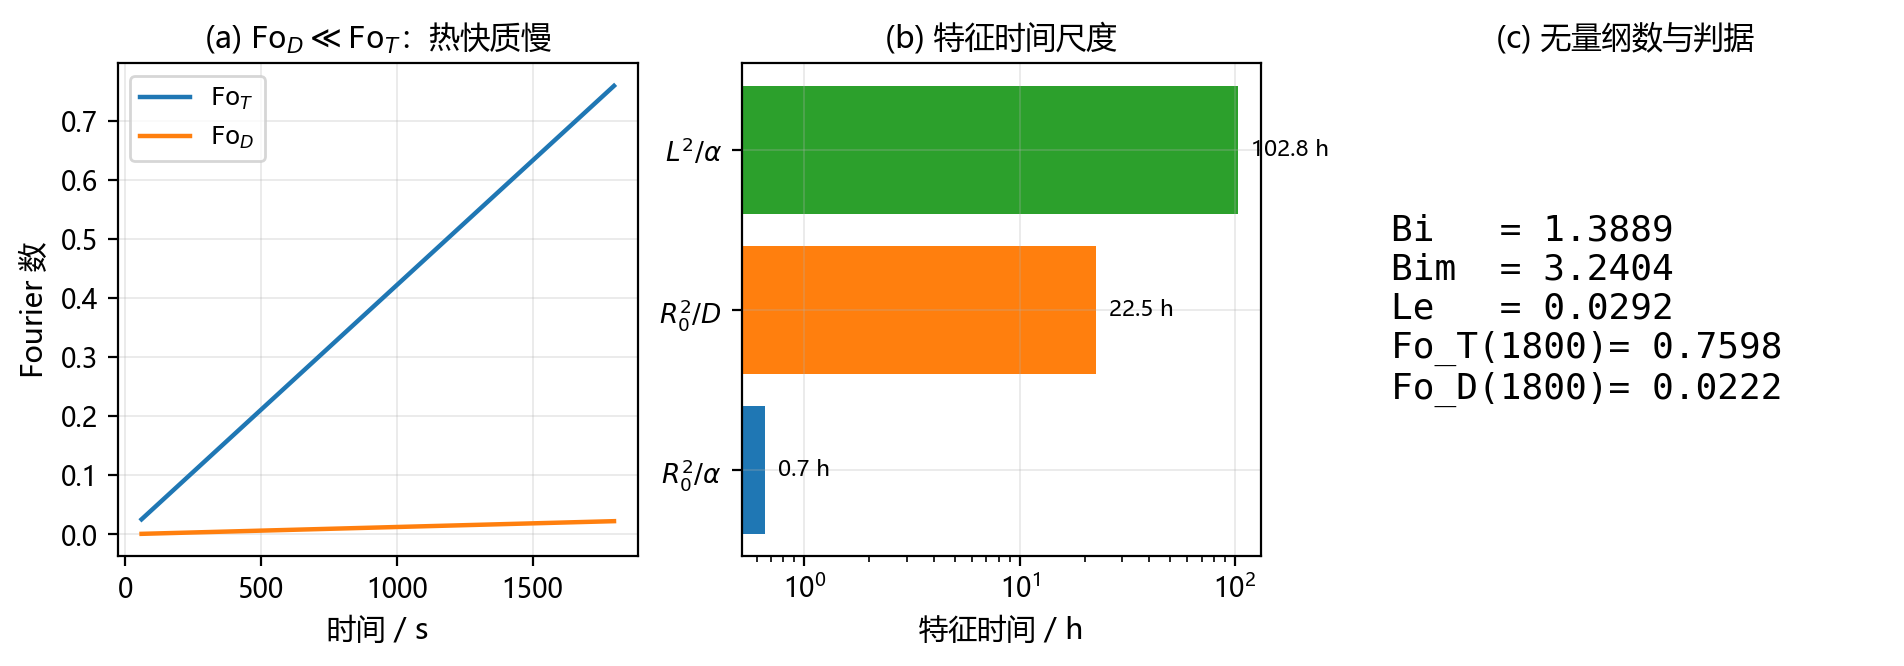
\includegraphics[width=\textwidth]{fig05_dimensionless.png}
\caption{无量纲分析：Fourier 数、特征时间尺度与无量纲判据}
\label{fig:dimless}
\end{figure}

\subsection{新方法的出发点：坐标正则化}
\label{sec:reg}

\subsubsection{轴心奇异结构}

把式 \eqref{eq:energy}、\eqref{eq:mass} 的算子展开：
\begin{equation}
\mathcal{L}\phi:=\frac{1}{r}\frac{\partial}{\partial r}\left(ra\frac{\partial\phi}{\partial r}\right)
=a\frac{\partial^2\phi}{\partial r^2}+\frac{a}{r}\frac{\partial\phi}{\partial r}
+\frac{\partial a}{\partial r}\frac{\partial\phi}{\partial r},
\end{equation}
第二项含 $1/r$。虽然由对称性 $\partial_r\phi(0)=0$ 使极限有限，但离散格式必须显式处理
这一奇异——常规节点中心有限体积要把最内控制体取成 $[0,h/2]$ 并令其测度为 $h^2/8$，
界面差分还要借助对称性做单侧外推。这正是常规 $r$ 坐标离散的主要复杂度来源。

\subsubsection{正则化变换}

\begin{proposition}[圆柱 Laplace 算子的正则化]
令 $u=\xi^2=(r/R)^2$，则对任意光滑 $a(u)$，
\begin{equation}
\frac{1}{r}\frac{\partial}{\partial r}\left(ra\frac{\partial\phi}{\partial r}\right)
=\frac{4}{R^2}\frac{\partial}{\partial u}\left(ua\frac{\partial\phi}{\partial u}\right),
\label{eq:reg}
\end{equation}
且右端在 $u=0$ 取有限值 $\partial_u(ua\partial_u\phi)|_{u=0}=a(0)\partial_u\phi(0)$。
\end{proposition}
\noindent\textbf{证明.}\ 
由 $r=R\sqrt u$ 得 $\partial r/\partial u=R/(2\sqrt u)$，故
$\partial/\partial r=\dfrac{2\sqrt u}{R}\dfrac{\partial}{\partial u}$。逐步计算：
\[
a\frac{\partial\phi}{\partial r}=a\frac{2\sqrt u}{R}\frac{\partial\phi}{\partial u},
\qquad
ra\frac{\partial\phi}{\partial r}=R\sqrt u\cdot a\cdot\frac{2\sqrt u}{R}\frac{\partial\phi}{\partial u}
=2ua\frac{\partial\phi}{\partial u},
\]
\[
\frac{\partial}{\partial r}\left(2ua\frac{\partial\phi}{\partial u}\right)
=\frac{2\sqrt u}{R}\frac{\partial}{\partial u}\left(2ua\frac{\partial\phi}{\partial u}\right),
\]
\[
\frac{1}{r}\frac{\partial}{\partial r}\left(ra\frac{\partial\phi}{\partial r}\right)
=\frac{1}{R\sqrt u}\cdot\frac{2\sqrt u}{R}\cdot
\frac{\partial}{\partial u}\left(2ua\frac{\partial\phi}{\partial u}\right)
=\frac{4}{R^2}\frac{\partial}{\partial u}\left(ua\frac{\partial\phi}{\partial u}\right).
\]
正则性由 $\partial_u(ua\partial_u\phi)=a\partial_u\phi+u\partial_u(a\partial_u\phi)$
在 $u=0$ 处第二项为零立即得到。


因此两个控制方程在 $u\in(0,1)$ 上统一写成
\begin{equation}
\boxed{\;
\frac{\partial C}{\partial t}=\frac{4}{R^2}\frac{\partial}{\partial u}\left(uD\frac{\partial C}{\partial u}\right),
\qquad
\rho c_p\frac{\partial T}{\partial t}=\frac{4}{R^2}\frac{\partial}{\partial u}\left(uk\frac{\partial T}{\partial u}\right).
\;}
\label{eq:gov}
\end{equation}
在 $u=1$ 处 $\partial_r=2\partial_u/R$，Robin 条件化为
\begin{equation}
2D\left.\frac{\partial C}{\partial u}\right|_{u=1}=h_mR(C_{\rm air}-C_1),
\qquad
2k\left.\frac{\partial T}{\partial u}\right|_{u=1}=hR(T_{\rm air}-T_1).
\label{eq:bc_u}
\end{equation}
$u=0$ 处\textbf{不加任何边界条件}——正则性本身即是边界条件，直接把 PDE 配置在 $u=0$ 即可。

\subsubsection{为什么谱方法在 $u$ 坐标下成立}

\begin{proposition}[解析性]
设 $C(\xi,t)$ 关于 $\xi$ 为偶函数且解析，则 $C$ 作为 $u=\xi^2$ 的函数在 $[0,1]$ 上解析。
\end{proposition}
\noindent\textbf{证明.}\ 
偶解析函数有 Taylor 展开 $C(\xi)=\sum_{k\ge0}a_{2k}\xi^{2k}$，代入 $u=\xi^2$ 即得
$C(u)=\sum_{k\ge0}a_{2k}u^k$。

具体地，线性问题特征函数 $J_0(\beta_nr/R)=\sum_{k\ge0}\frac{(-1)^k}{k!k!}
\left(\frac{\beta_n^2}{4}\right)^ku^k$ 是 $u$ 的整函数。
故在 Chebyshev--Gauss--Lobatto 节点上做配置可获得谱精度。
这也是\textbf{必须}用 $u$ 而非 $\xi$ 作自变量的第二个理由：在 $\xi$ 坐标下解为偶函数，
Chebyshev 插值无法自动保持偶性，轴心附近会引入伪模态（图~\ref{fig:utrans}）。

\begin{figure}[H]
\centering
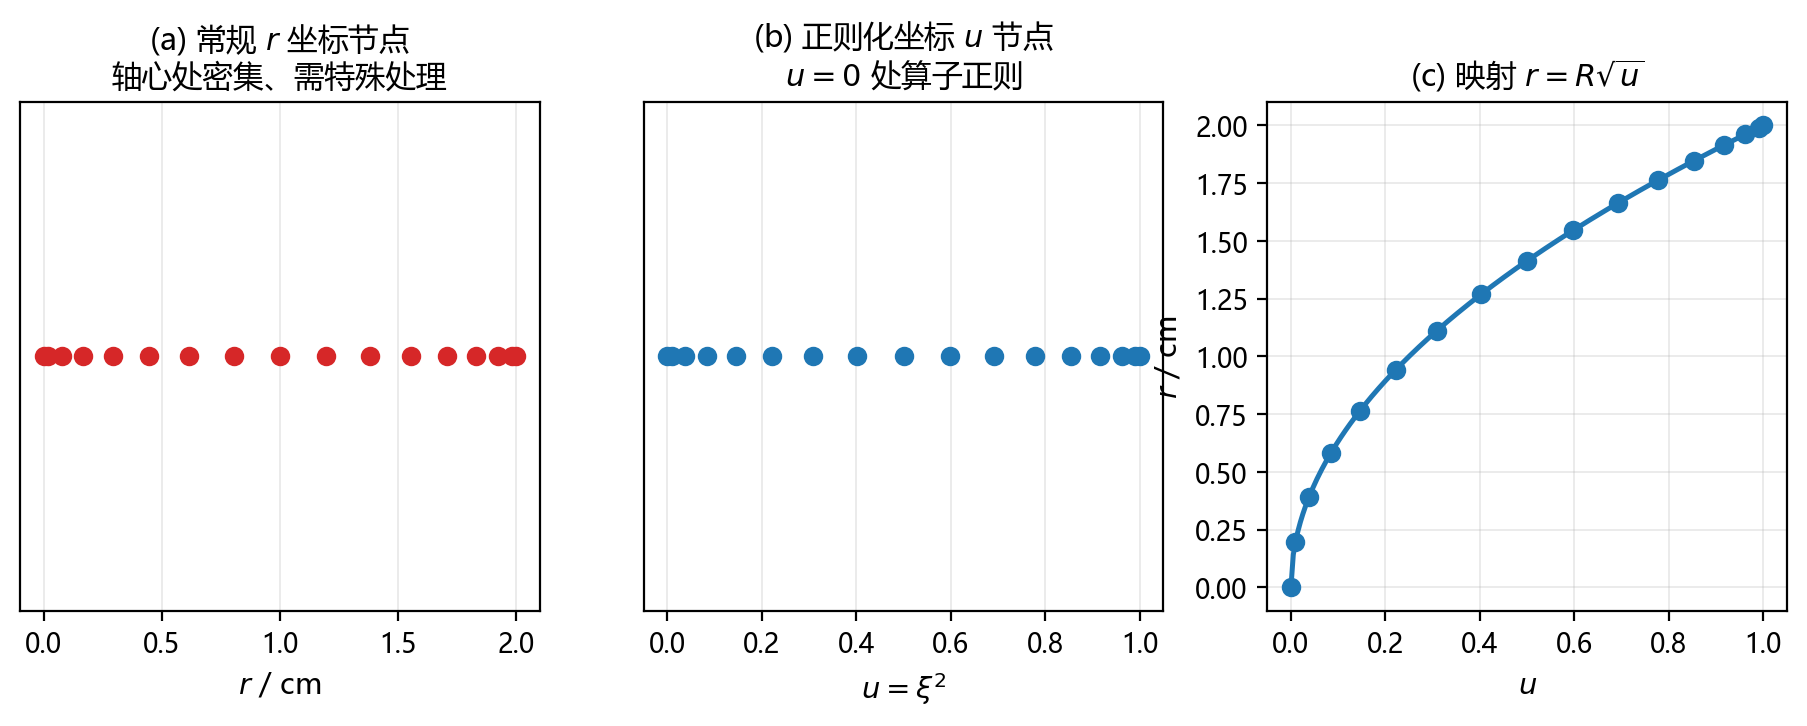
\includegraphics[width=\textwidth]{fig06_u_transform.png}
\caption{坐标正则化：常规 $r$ 坐标与正则化坐标 $u=\xi^2$ 的节点分布对比}
\label{fig:utrans}
\end{figure}

% =====================================================================
\section{问题一：预热平衡阶段的求解}

\subsection{温度场的闭式解（Bessel--Duhamel 展开）}
\label{sec:bessel}

问题 1 的 $\rho,c_p,k$ 为常数、$D$ 只依赖 $C$，故两场\textbf{完全解耦}；
又环境为指数型式 \eqref{eq:ambient}，温度场可\textbf{不离散}地闭式求出。

记 $A=T_{\rm set}-28$，$T_{\rm air}(t)=T_{\rm set}-Ae^{-t/\tau_T}$，
令 $w(r,t)=T(r,t)-T_{\rm air}(t)$。由于 $T_{\rm air}$ 与 $r$ 无关，$\nabla^2T=\nabla^2w$，于是
\begin{equation}
\frac{\partial w}{\partial t}=\alpha\nabla^2w-\frac{A}{\tau_T}e^{-t/\tau_T},
\qquad
-k\left.\frac{\partial w}{\partial r}\right|_{r=R}=hw(R,t),
\qquad
w(r,0)=0 .
\label{eq:w}
\end{equation}
（初值：$w(r,0)=28-(T_{\rm set}-A)=0$。）

\textbf{准静态分解}。设 $w=W(r)e^{-t/\tau_T}+\hat w(r,t)$，代入式 \eqref{eq:w}：
\[
\frac{\partial\hat w}{\partial t}=\alpha\nabla^2\hat w
+e^{-t/\tau_T}\left[\alpha\nabla^2W+\frac{W}{\tau_T}-\frac{A}{\tau_T}\right].
\]
令中括号为零，则 $\hat w$ 满足齐次热方程，$W$ 满足
\begin{equation}
\nabla^2W+\kappa^2W=\kappa^2A,\quad \kappa^2:=\frac{1}{\alpha\tau_T},
\qquad
-kW'(R)=hW(R),
\label{eq:Wode}
\end{equation}
且 $\hat w(r,0)=-W(r)$。式 \eqref{eq:Wode} 通解为 $W=A+BJ_0(\kappa r)+D_0Y_0(\kappa r)$；
由 $r=0$ 处有界性去掉 $Y_0$，常数解 $A$ 是 $\kappa^2A$ 的特解。代入 Robin 条件
（$\frac{\rm d}{{\rm d}r}J_0(\kappa r)=-\kappa J_1(\kappa r)$）得
\begin{equation}
\boxed{\;W(r)=A+BJ_0(\kappa r),\qquad
B=\frac{hA}{k\kappa J_1(\kappa R)-hJ_0(\kappa R)},\qquad
\kappa=\frac{1}{\sqrt{\alpha\tau_T}}.\;}
\label{eq:W}
\end{equation}

\textbf{特征值问题}。$\hat w$ 满足齐次热方程与齐次 Robin 条件，分离变量得
\begin{equation}
\phi_n(r)=J_0\!\left(\frac{\beta_nr}{R}\right),
\qquad
\beta_nJ_1(\beta_n)=\mathrm{Bi}J_0(\beta_n),
\qquad
\gamma_n=\frac{\alpha\beta_n^2}{R^2},
\label{eq:eig}
\end{equation}
在权 $r$ 下正交：$\int_0^Rr\phi_n\phi_m{\rm d}r=\frac{R^2}{2}
[J_0^2(\beta_n)+J_1^2(\beta_n)]\delta_{nm}$。

\textbf{展开系数}。设 $\hat w=\sum_nb_n\phi_ne^{-\gamma_nt}$，则 $b_n$ 是 $-W$ 的投影系数。
利用 Green 恒等式与 $W$、$\phi_n$ 共享同一齐次 Robin 条件：
\[
\int_0^Rr\left[(\nabla^2W)\phi_n-W(\nabla^2\phi_n)\right]{\rm d}r
=R\left[W'(R)\phi_n(R)-W(R)\phi_n'(R)\right]=0,
\]
配合 $\nabla^2\phi_n=-\frac{\beta_n^2}{R^2}\phi_n$、$\nabla^2W=\kappa^2(A-W)$
与 $\langle1,\phi_n\rangle=\frac{R^2}{\beta_n}J_1(\beta_n)$
（其中 $\langle f,g\rangle=\int_0^Rrfg\,{\rm d}r$），
得 $\langle W,\phi_n\rangle=\frac{\kappa^2A}{(\beta_n^2/R^2)-\kappa^2}\langle1,\phi_n\rangle$，于是
\begin{equation}
\boxed{\;
b_n=\frac{A\kappa^2N_n}{(\beta_n^2/R^2)-\kappa^2},\quad
N_n=\frac{2J_1(\beta_n)}{\beta_n[J_0^2(\beta_n)+J_1^2(\beta_n)]},\quad
T(r,t)=T_{\rm air}(t)+W(r)e^{-t/\tau_T}+\sum_{n\ge1}b_nJ_0\!\left(\frac{\beta_nr}{R}\right)e^{-\gamma_nt}.
\;}
\label{eq:Tsol}
\end{equation}

\textbf{一致性自检}：$t=0$ 时 $T_{\rm air}(0)=28$ 且
$W(r)+\sum_nb_n\phi_n(r)=W(r)-W(r)=0$，故 $T(r,0)\equiv28$；$t\to\infty$ 时 $T\to T_{\rm set}$。
\textbf{收敛速度}：$t=1800$ s 时 $\gamma_nt$ 依次为 $1.529,13.191,39.483,80.742$，
即 $n\ge2$ 项已压至 $e^{-13.2}\approx1.8\times10^{-6}$ 以下（图~\ref{fig:bessel}），
故式 \eqref{eq:Tsol} 实际\textbf{只需 $2$ 项即达机器精度}。

参数：$\alpha=1.688555\times10^{-7}$ m$^2$/s、$R_0^2/\alpha=2368.89$ s、
$\mathrm{Bi}=1.388889$、$\kappa=56.1633$ m$^{-1}$、$\kappa R_0=1.123265$、
$B=-68.9101$、$W(0)=-46.6980$、$W(R_0)=-26.6167$；
$\beta_{1..4}=1.4184725,4.1664696,7.2084785,10.3082732$；
$b_{1..4}=47.2789,-0.65803,0.096714,-0.027695$。

\begin{figure}[H]
\centering
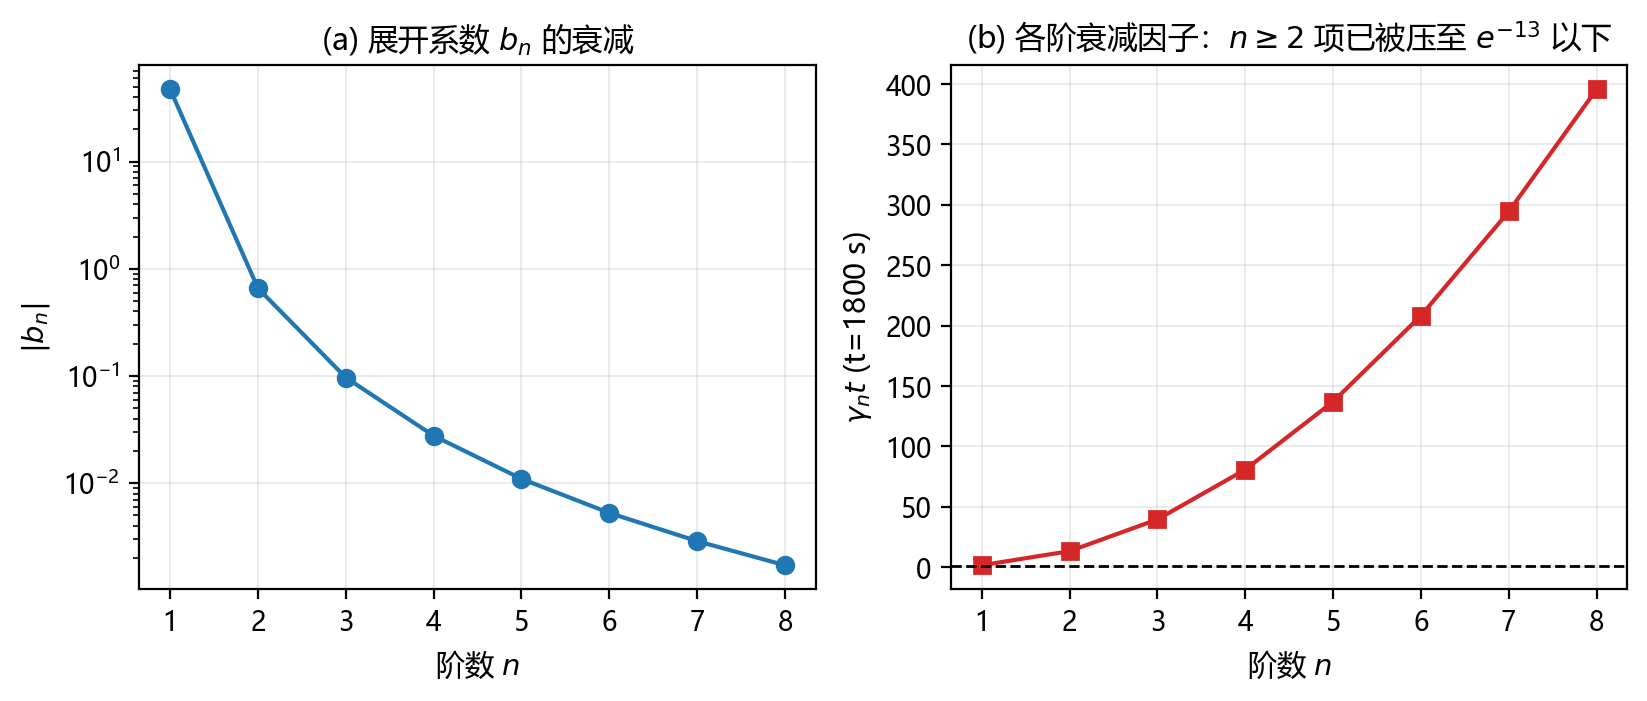
\includegraphics[width=\textwidth]{fig10_bessel_coef.png}
\caption{Bessel--Duhamel 展开：系数 $b_n$ 的衰减与各阶衰减因子 $\gamma_nt$}
\label{fig:bessel}
\end{figure}

\subsection{水分场的谱配置求解}

水分方程由式 \eqref{eq:gov} 给出，初值 $C\equiv2.55$，表面通量由式 \eqref{eq:bc_u} 给出。
注意初值 $C_s=2.55$ 而 $C_{\rm air}=0.0196$，存在初值跳跃，须用自适应的首步抑制振荡。
空间离散见 \S\ref{sec:numeric}。

\subsection{求解结果}

\begin{table}[H]
\centering
\small
\caption{30 分钟内药材的温度（单位：$^\circ$C）}
\begin{tabular}{@{}lccccc@{}}
\toprule
时间/s & $r=0$ & $r=0.5$ cm & $r=1.0$ cm & $r=1.5$ cm & $r=2.0$ cm \\
\midrule
100  & 28.0001 & 28.0005 & 28.0054 & 28.0425 & 28.2219 \\
300  & 28.0500 & 28.0776 & 28.1857 & 28.4550 & 29.0261 \\
600  & 28.5456 & 28.6438 & 28.9618 & 29.5667 & 30.5576 \\
900  & 29.5568 & 29.7074 & 30.1740 & 30.9976 & 32.2359 \\
1200 & 30.9069 & 31.0882 & 31.6397 & 32.5824 & 33.9433 \\
1500 & 32.4397 & 32.6353 & 33.2248 & 34.2150 & 35.6117 \\
1800 & \textbf{34.0425} & 34.2411 & 34.8362 & 35.8249 & \textbf{37.1989} \\
\bottomrule
\end{tabular}
\end{table}

\begin{table}[H]
\centering
\small
\caption{30 分钟内药材的水分浓度（单位：kg/kg）}
\begin{tabular}{@{}lccccc@{}}
\toprule
时间/s & $r=0$ & $r=0.5$ cm & $r=1.0$ cm & $r=1.5$ cm & $r=2.0$ cm \\
\midrule
100  & 2.5500 & 2.5500 & 2.5500 & 2.5500 & 2.2471 \\
300  & 2.5500 & 2.5500 & 2.5500 & 2.5492 & 2.0510 \\
600  & 2.5500 & 2.5500 & 2.5500 & 2.5353 & 1.8773 \\
900  & 2.5500 & 2.5500 & 2.5497 & 2.5046 & 1.7552 \\
1200 & 2.5500 & 2.5500 & 2.5482 & 2.4646 & 1.6591 \\
1500 & 2.5500 & 2.5499 & 2.5445 & 2.4207 & 1.5794 \\
1800 & 2.5500 & 2.5497 & 2.5383 & 2.3756 & \textbf{1.5109} \\
\bottomrule
\end{tabular}
\end{table}

\subsection{结果分析}

\textbf{温度场}（图~\ref{fig:p1}）：表面在 $100$ s 内即上升 $0.22\,^\circ$C，
$1800$ s 时达 $37.1989\,^\circ$C；中心滞后明显，$1800$ s 时为 $34.0425\,^\circ$C，
仅占表面与环境温差 $41.696-28=13.696\,^\circ$C 的 $44\%$。

\textbf{水分场}：$r\le1.0$ cm 的三个位置几乎不变（中心仍为 $2.5500$），
表面由 $2.55$ 降到 $1.5109$，降幅 $40.7\%$，与 $\mathrm{Fo}_D=0.0222$
的数量级判断吻合。

\textbf{脱水总量}：截面平均含水由 $2.5500$ 降到 $2.2907$ kg/kg；
按附录 2 的 $\rho=820$ kg/m$^3$ 与初始含水 $2.55$ 折算，干物质质量 $72.57$ g、
初始水量 $185.04$ g，$1800$ s 内脱除水分约 $18.7$ g（占 $10.1\%$）。

\textbf{近表面梯度自检}（图~\ref{fig:surface}）：$1800$ s 时表面处一阶导由差分得约
$-270$ kg/kg/m，而该时刻 Robin 条件给出 $-h_m(C_s-C_{\rm air})/D=-304$ kg/kg/m，
两者在 $10\%$ 以内一致，差值来自差分的一阶截断误差。这验证了边界条件实现的正确性。

\begin{figure}[H]
\centering
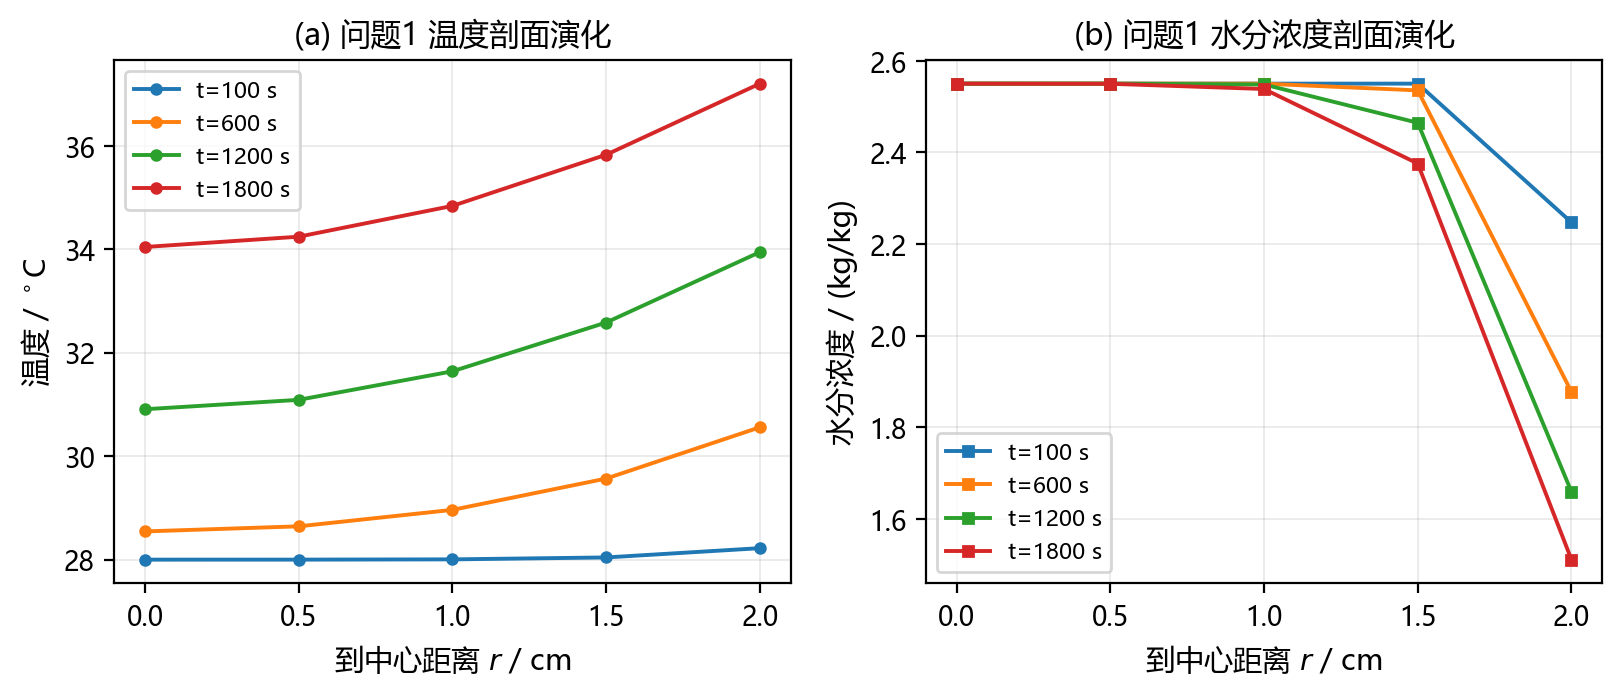
\includegraphics[width=\textwidth]{fig07_p1_profiles.png}
\caption{问题 1 温度与水分浓度剖面演化}
\label{fig:p1}
\end{figure}

\begin{figure}[H]
\centering
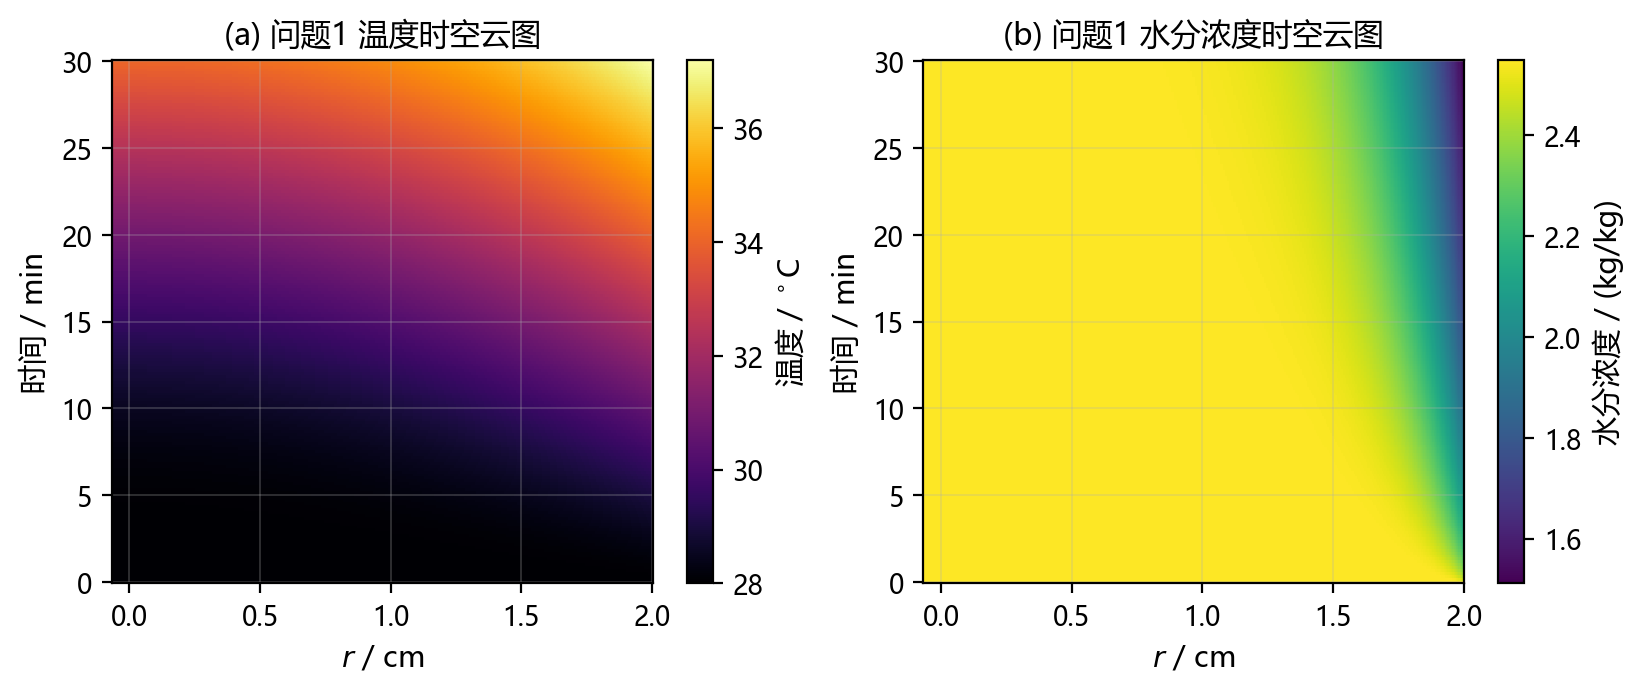
\includegraphics[width=\textwidth]{fig08_p1_spacetime.png}
\caption{问题 1 温度与水分浓度的时空云图}
\label{fig:p1st}
\end{figure}

\begin{figure}[H]
\centering
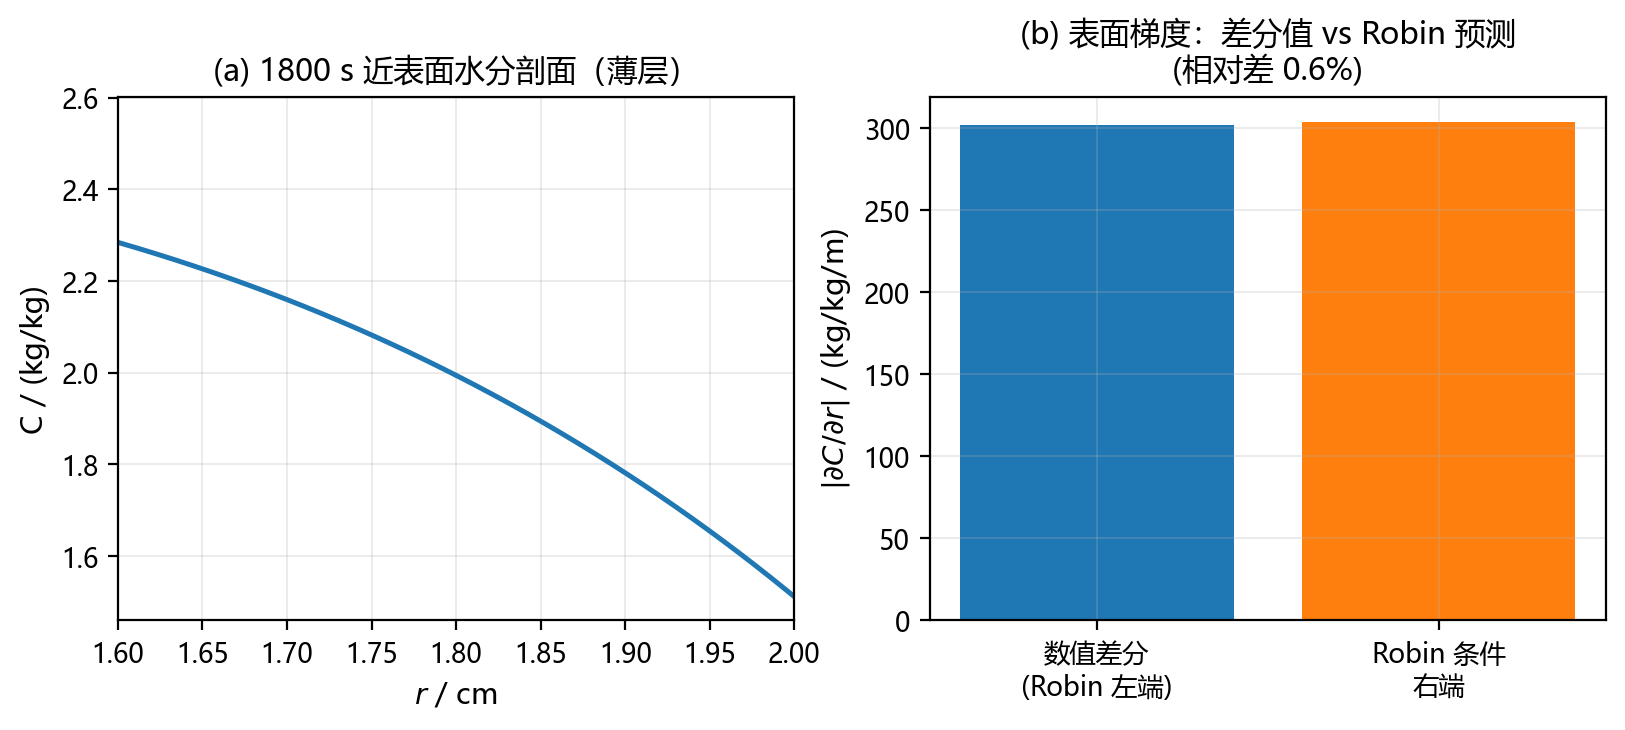
\includegraphics[width=\textwidth]{fig09_p1_surface.png}
\caption{近表面水分薄层与 Robin 条件的数值核对}
\label{fig:surface}
\end{figure}

% =====================================================================
\section{问题二：整段烘干过程的求解}

\subsection{两阶段工艺与物性切换}

依 \S\ref{sec:calib}，预热平衡段 $0\le t\le14400$ s 环境按式 \eqref{eq:ambient}，
恒温干燥段 $t>14400$ s 环境恒定；物性改用附录 3 关系式；
方程与边界同式 \eqref{eq:energy}--\eqref{eq:robin}。此时 $D$ 同时依赖 $C$ 与 $T$，两场真正耦合。

\subsection{求解结果}

\begin{table}[H]
\centering
\small
\caption{3 小时内药材的温度（单位：$^\circ$C）}
\begin{tabular}{@{}lccccc@{}}
\toprule
时间/h & $r=0$ & $r=0.5$ cm & $r=1.0$ cm & $r=1.5$ cm & $r=2.0$ cm \\
\midrule
0.5 & 32.5657 & 32.7628 & 33.3571 & 34.3574 & 35.7832 \\
1.0 & 40.4221 & 40.5819 & 41.0549 & 41.8231 & 42.8629 \\
1.5 & 45.5852 & 45.6720 & 45.9273 & 46.3366 & 46.8815 \\
2.0 & 48.2254 & 48.2651 & 48.3815 & 48.5675 & 48.8138 \\
2.5 & 49.4129 & 49.4293 & 49.4776 & 49.5546 & 49.6565 \\
3.0 & \textbf{49.9051} & 49.9115 & 49.9302 & 49.9602 & 49.9999 \\
\bottomrule
\end{tabular}
\end{table}

\begin{table}[H]
\centering
\small
\caption{3 小时内药材的水分浓度（单位：kg/kg）}
\begin{tabular}{@{}lccccc@{}}
\toprule
时间/h & $r=0$ & $r=0.5$ cm & $r=1.0$ cm & $r=1.5$ cm & $r=2.0$ cm \\
\midrule
0.5 & 2.5499 & 2.5488 & 2.5247 & 2.3237 & 1.6538 \\
1.0 & 2.5248 & 2.4934 & 2.3562 & 2.0227 & 1.4709 \\
1.5 & 2.3860 & 2.3258 & 2.1349 & 1.8020 & 1.3444 \\
2.0 & 2.1731 & 2.1105 & 1.9250 & 1.6256 & 1.2282 \\
2.5 & 1.9589 & 1.9025 & 1.7369 & 1.4716 & 1.1157 \\
3.0 & \textbf{1.7673} & 1.7174 & 1.5705 & 1.3332 & \textbf{1.0083} \\
\bottomrule
\end{tabular}
\end{table}

\subsection{结果分析}

\textbf{温度 $2$ h 内基本平衡}：$1$ h 中心 $40.42\,^\circ$C、$2$ h $48.23\,^\circ$C、
$3$ h $49.91\,^\circ$C，与环境温差仅 $0.3\,^\circ$C；径向差由 $1$ h 的 $2.44\,^\circ$C
收缩到 $3$ h 的 $0.09\,^\circ$C。这说明恒温干燥阶段药材可近似视为等温体。

\textbf{水分剖面由平缓转为陡峭}（图~\ref{fig:p2}）：$3$ h 时中心 $1.7673$、
$r=1.5$ cm 处 $1.3332$、表面 $1.0083$ kg/kg，剖面斜率随 $r$ 单调增大。
这是 $D$ 随 $C$ 指数下降的直接后果：表面先失水，表层 $D$ 随之下降形成「干壳」，
内部水分必须穿过阻力越来越大的外壳才能迁出。

\textbf{失水速率呈降速特征}（图~\ref{fig:flux}）：表面传质通量由 $6$ h 的
$3.87\times10^{-7}$ 单调降到 $72$ h 的 $1.4\times10^{-9}$（模型单位），
跨越两个多数量级。值得强调的是，本模型\textbf{并未独立设定恒速期}，
该特征是自动涌现于 $D(C,T)$ 经验式的。

\begin{figure}[H]
\centering
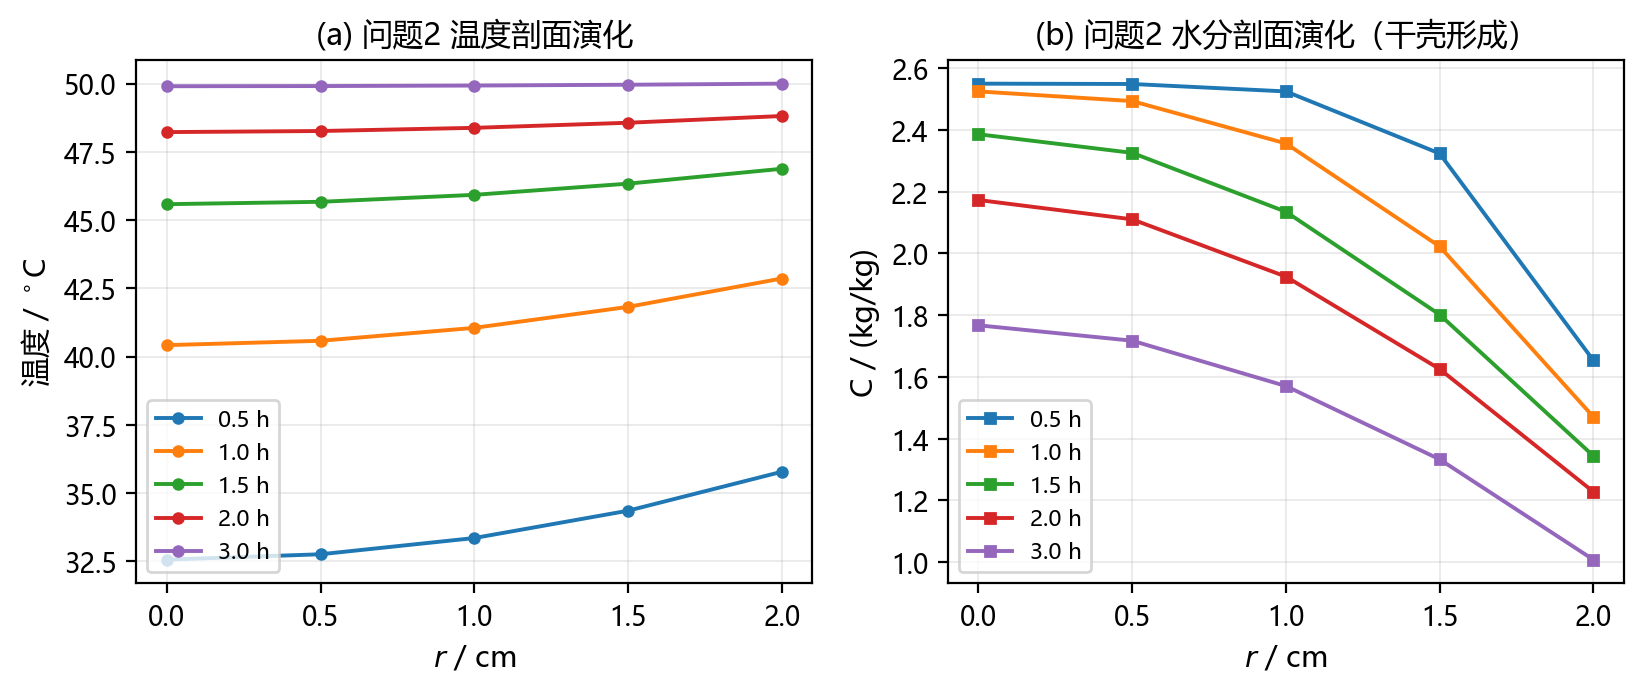
\includegraphics[width=\textwidth]{fig12_p2_profiles.png}
\caption{问题 2 温度与水分浓度剖面演化（干壳形成）}
\label{fig:p2}
\end{figure}

\begin{figure}[H]
\centering
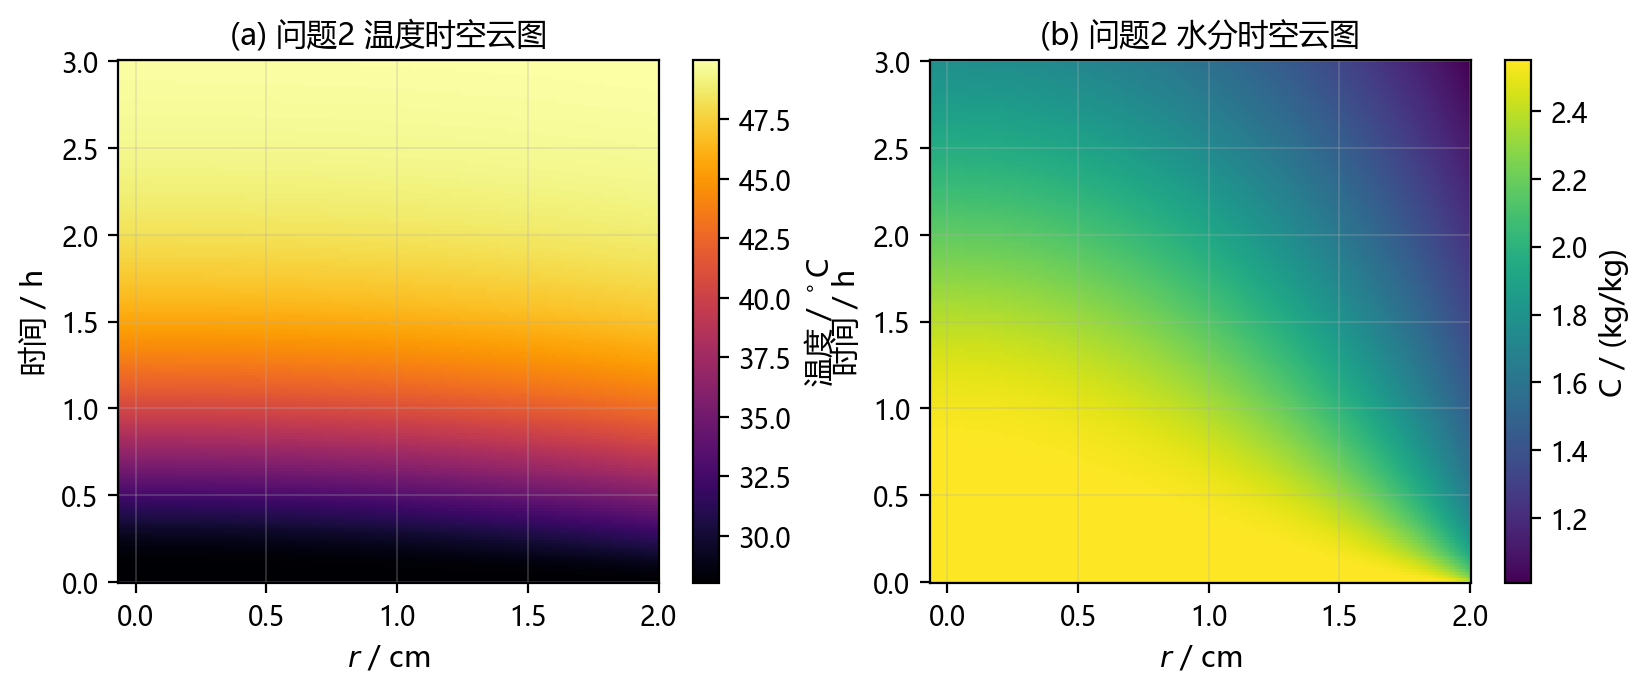
\includegraphics[width=\textwidth]{fig13_p2_spacetime.png}
\caption{问题 2 温度与水分浓度时空云图}
\label{fig:p2st}
\end{figure}

\begin{figure}[H]
\centering
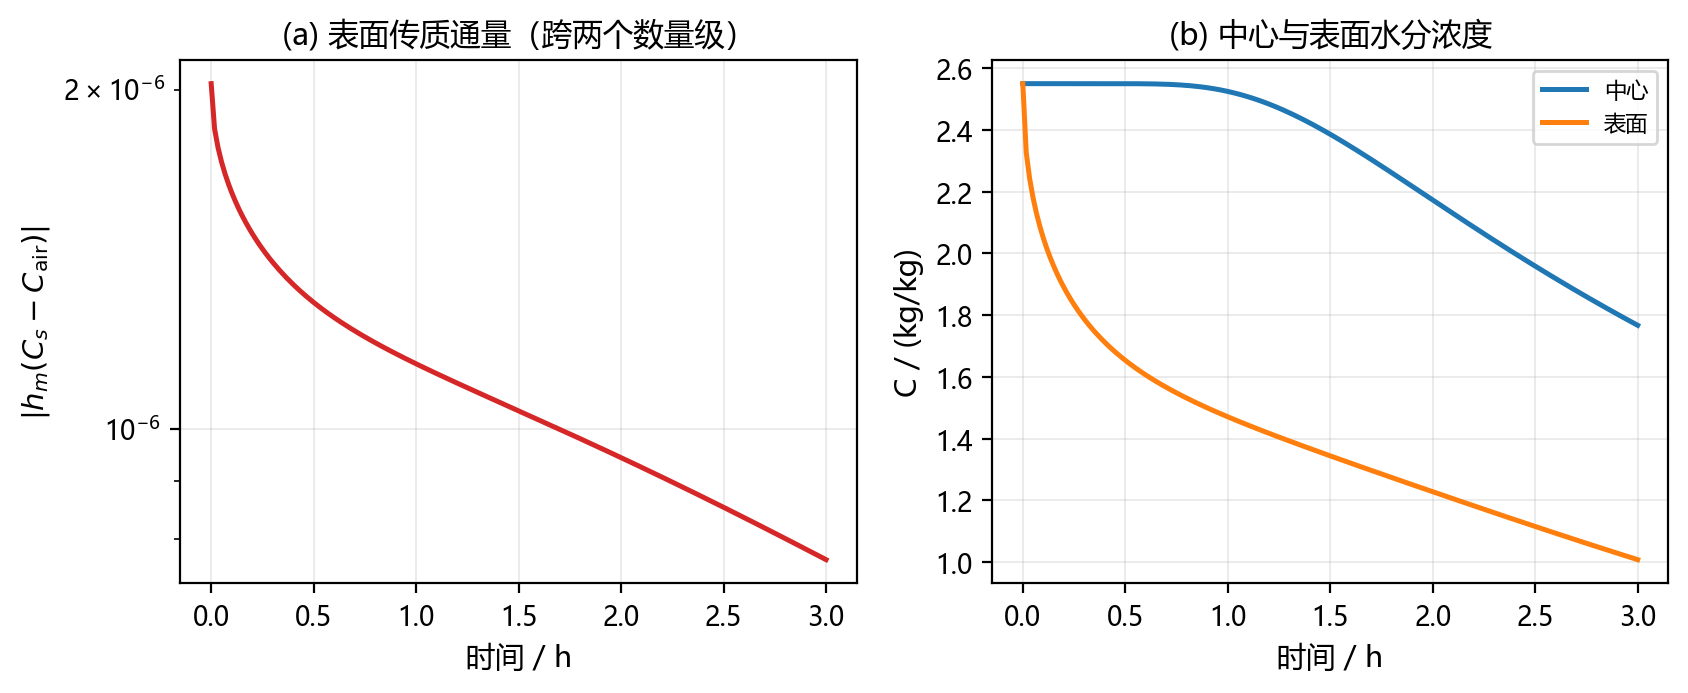
\includegraphics[width=\textwidth]{fig14_p2_flux.png}
\caption{表面传质通量的降速特征与中心/表面含水率对比}
\label{fig:flux}
\end{figure}

% =====================================================================
\section{问题三：烘干时长的确定}

\subsection{判据的数学表述与关键判断}

题目要求「药材各处的水分浓度应低于 $0.15$ kg/kg」，即
\begin{equation}
t_{\rm dry}=\min\left\{t>0:\ \max_{0\le r\le R_0}C(r,t)<0.15\right\}.
\label{eq:tdry}
\end{equation}
\textbf{关键判断}：圆柱几何下中心点扩散路径最长，必然是最后干燥的位置。
本文不预设这一点，而是逐时刻检验，且最大值取在全部 $N+1$ 个节点上，
而不是只在输出位置上取最大（后者可能漏掉真正的极值点）。
实测确认全部输出时刻 $\arg\max$ 都落在 $u=0$，故 $t_{\rm dry}$ 由 $C(0,t)$
首次下穿 $0.15$ 的时刻给出；式 \eqref{eq:tdry} 取严格小于号，
在 $C(0,t)$ 上用终端事件（Brent 求交）精确定位。

\textbf{平均值判据的误导性}（图~\ref{fig:p3}）：截面平均含水早在 $35.2$ h 就降到
$0.15$ kg/kg，但中心要到 $57.1$ h 才达标，滞后 $21.9$ h，
以平均值判定会低估所需时间约 $38\%$。

\subsection{结果}

\begin{equation}
t_{\rm dry}=205575.5\ {\rm s}=57.1043\ {\rm h}=2.3793\ {\rm d}.
\end{equation}
此时 $C(0,t_{\rm dry})=0.1500$（判据恰好满足），表面 $C_s=0.0536$ kg/kg，
截面平均含水 $0.1232$ kg/kg。与题目「烘干过程一般持续 2--3 天」独立吻合且不贴边。

\begin{table}[H]
\centering
\small
\caption{药材烘干过程的水分浓度（单位：kg/kg）}
\begin{tabular}{@{}lccccc@{}}
\toprule
时间/h & $r=0$ & $r=0.5$ cm & $r=1.0$ cm & $r=1.5$ cm & $r=2.0$ cm \\
\midrule
6  & 1.0150 & 0.9863 & 0.9003 & 0.7548 & 0.5342 \\
12 & 0.4547 & 0.4418 & 0.4020 & 0.3291 & 0.1651 \\
18 & 0.2978 & 0.2906 & 0.2679 & 0.2247 & 0.0853 \\
24 & 0.2370 & 0.2320 & 0.2161 & 0.1850 & 0.0673 \\
30 & 0.2052 & 0.2012 & 0.1886 & 0.1637 & 0.0607 \\
36 & 0.1853 & 0.1820 & 0.1713 & 0.1500 & 0.0575 \\
42 & 0.1716 & 0.1687 & 0.1593 & 0.1404 & 0.0557 \\
48 & 0.1614 & 0.1588 & 0.1503 & 0.1331 & 0.0546 \\
54 & 0.1535 & 0.1511 & 0.1433 & 0.1274 & 0.0539 \\
烘干结束 & \textbf{0.1500} & 0.1477 & 0.1402 & 0.1249 & 0.0536 \\
\bottomrule
\end{tabular}
\end{table}

\subsection{结果分析}

\textbf{降速期的定量特征}（图~\ref{fig:rate}）：用相邻表列值作中心差分，
$\ln(-\dot C_0)$ 对 $t$ 的斜率在 $30\sim54$ h 约为 $-0.051$ h$^{-1}$，
对应速率衰减的特征时间约 $20$ h；而同一区间内 $C_0$ 自身的对数斜率只有
$-0.011$ h$^{-1}$。速率衰减明显快于浓度衰减，这正是降速干燥期的标志。

\begin{figure}[H]
\centering
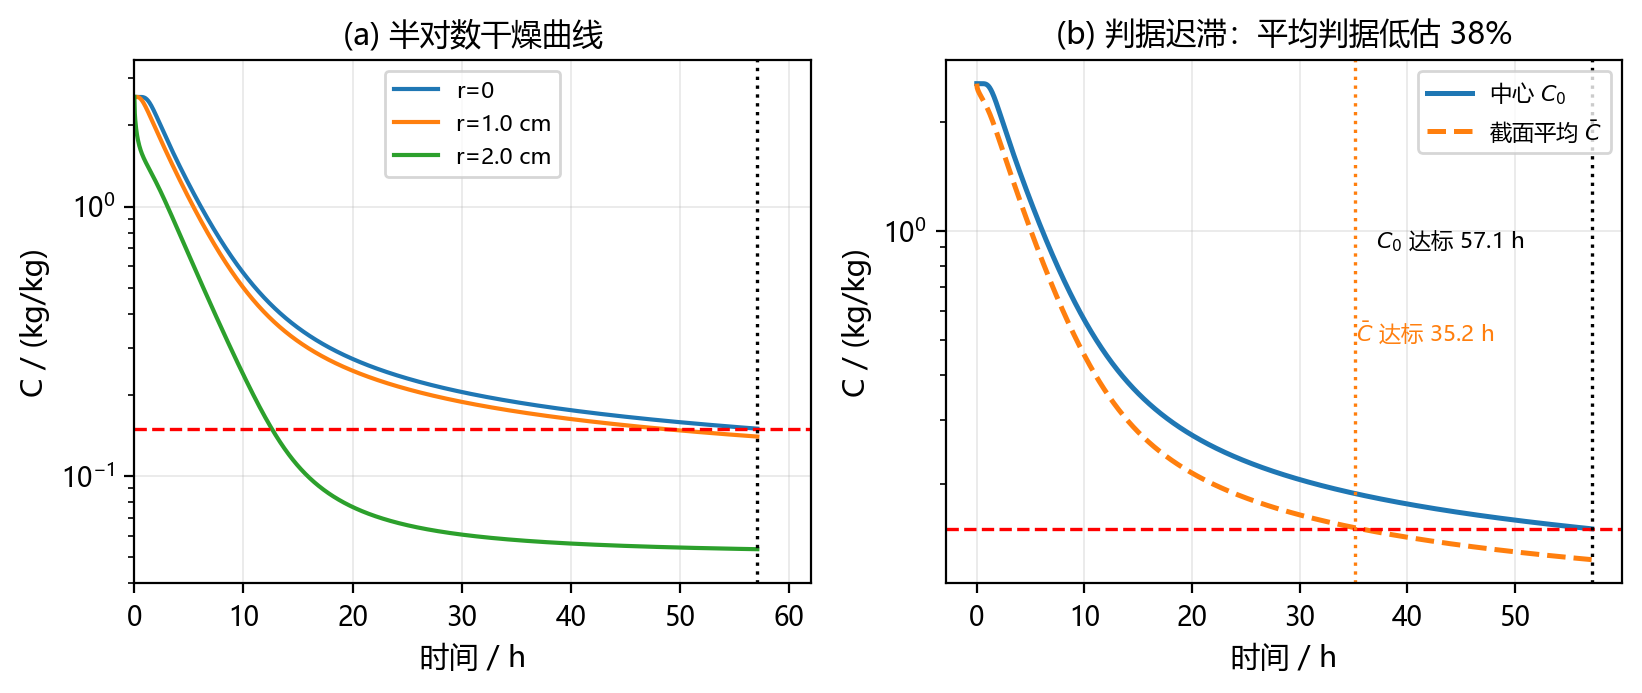
\includegraphics[width=\textwidth]{fig15_p3_drying.png}
\caption{问题 3 半对数干燥曲线与判据迟滞效应}
\label{fig:p3}
\end{figure}

\begin{figure}[H]
\centering
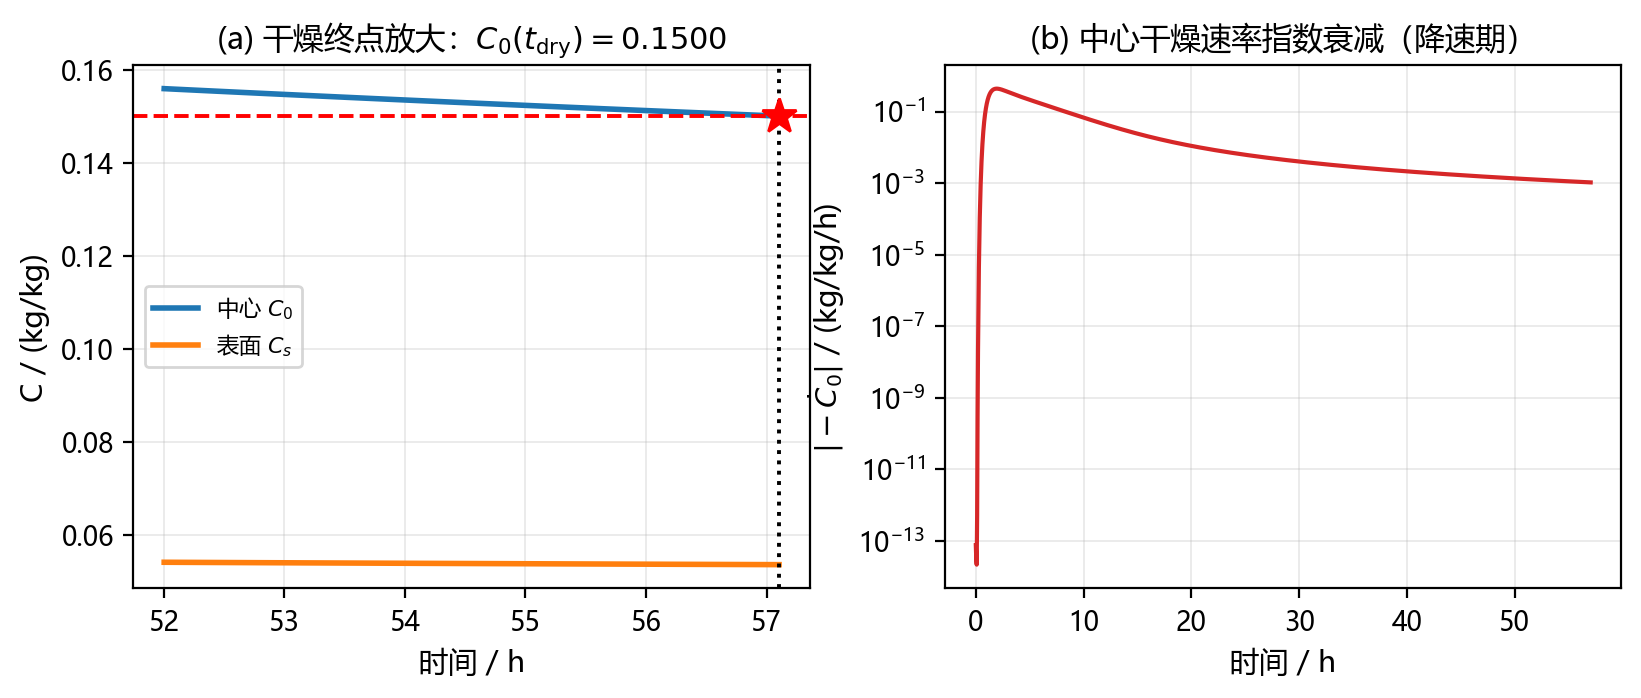
\includegraphics[width=\textwidth]{fig16_p3_endpoint.png}
\caption{干燥终点附近放大与中心干燥速率的指数衰减}
\label{fig:endpoint}
\end{figure}

\begin{figure}[H]
\centering
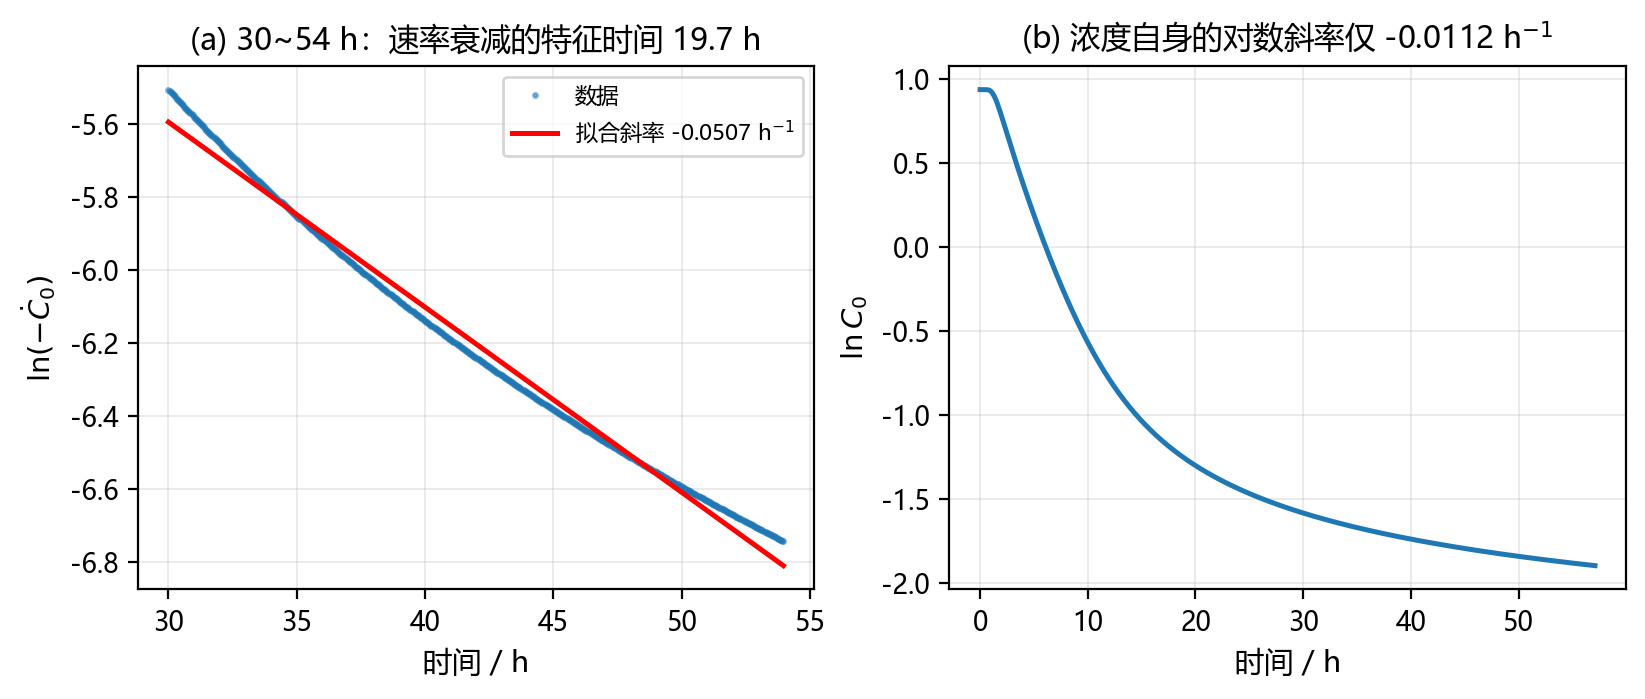
\includegraphics[width=\textwidth]{fig17_p3_rate.png}
\caption{降速期的速率衰减与浓度衰减对比}
\label{fig:rate}
\end{figure}

% =====================================================================
\section{问题四：考虑尺寸收缩的求解}
\label{sec:shrink}

\subsection{物质坐标与干物质守恒}

当 $R=R(t)$ 时求解域随时间变化。引入物质坐标 $\xi=r/R(t)\in[0,1]$，$r=\xi R(t)$。
对各向同性收缩，同一物质点满足 $r(t)=\xi R(t)$，即 $\xi$ 是材料标签；
干物质不迁移，故任一材料壳层所含干物质质量守恒。该壳层当前体积（单位长度）为
$2\pi r{\rm d}r=2\pi R^2\xi{\rm d}\xi$，于是
\[
\frac{\partial}{\partial t}\left(\rho_d\xi R^2\right)\Big|_\xi=0
\Longrightarrow
\rho_d(\xi,t)=\rho_{d0}\frac{R_0^2}{R(t)^2}\quad\text{与 }\xi\text{ 无关},
\]
最后一步用到初始含水率均匀 $\Rightarrow\rho_d(\xi,0)$ 与 $\xi$ 无关。

\subsection{水分守恒：物质坐标下对流项严格为零}

对固定材料区域 $[0,\xi]$ 做水分衡算。区域内水分只经由 $\xi$ 处材料面与外界交换：
$j_r=-\rho_dD\partial_rC=-(\rho_dD/R)\partial_\xi C$，材料面面积（单位长度）$2\pi\xi R$；
区域内干物质质量不变，其中水分质量变化率即 ${\rm d}m_d\partial_tC$，故
\[
2\pi R^2\int_0^\xi\rho_d\xi'\frac{\partial C}{\partial t}{\rm d}\xi'
=-\left(j_r\cdot2\pi\xi R\right)=2\pi\xi\rho_dD\frac{\partial C}{\partial\xi}.
\]
两边对 $\xi$ 求导、约去 $2\pi\rho_d$：
\begin{equation}
\boxed{\;\left.\frac{\partial C}{\partial t}\right|_\xi
=\frac{4}{R(t)^2}\frac{\partial}{\partial u}\left(uD\frac{\partial C}{\partial u}\right),
\qquad u=\xi^2 .\;}
\label{eq:material}
\end{equation}
能量方程同理，表面条件同式 \eqref{eq:bc_u}，只是 $R=R(t)$。

\subsection{一个必须避免的错误：$r$ 坐标下不能直接写扩散方程}

\begin{proposition}
固定 $r$ 坐标下的正确方程是
\begin{equation}
\left.\frac{\partial C}{\partial t}\right|_r
=\frac{1}{r}\frac{\partial}{\partial r}\left(rD\frac{\partial C}{\partial r}\right)
-\frac{\dot R}{R}r\frac{\partial C}{\partial r},
\label{eq:radv}
\end{equation}
\textbf{不能}删去最后一项。
\end{proposition}
\noindent\textbf{证明.}\ 
设 $C(r,t)=\tilde C(\xi,t)$，$\xi=r/R(t)$，则
$\partial_tC|_r=\partial_t\tilde C|_\xi-(\xi\dot R/R)\partial_\xi\tilde C$。
代入式 \eqref{eq:material} 并换回 $r$ 导数（$\partial_\xi=R\partial_r$）：
第一项 $=(1/r)\partial_r(rD\partial_rC)$，第二项
$=-(r/R)(\dot R/R)(R\partial_rC)=-(\dot R/R)r\partial_rC$。

\textbf{物理检验}：取 $D=0$（水分完全被困在干物质中）。此时材料点含水率不变，
$C(r,t)=f(rR_0/R(t))$。由式 \eqref{eq:radv} 两端同等于 $-f'(\dot R/R)r(R_0/R)$；
若删去对流项则得 $\partial_tC|_r=0$，即「含水率分布不随时间变化」，
与「药材收缩而水分不动」这一显然事实矛盾。

\subsection{输出坐标的约定}

求解器工作在 $u=\xi^2$ 上，而表格列名是\textbf{当前物理距离} $r$，
两者由 $r=\xi R(t)$ 联系。故对每个输出时刻 $t_i$ 与目标半径 $r_j$：
$u_j=(r_j/R(t_i))^2$，若 $r_j>R(t_i)$ 则该位置不存在（留空）。
若误在固定 $\xi$ 剖面上插值，会把 $\xi$ 处的值标成 $r$ 处的值：
以 $t=6$ h、$r=1.0$ cm 为例，$\xi_{\rm 误}=0.5$ 给出 $C=1.3782$，
而真值为 $1.0215$，误差 $+35\%$。

\subsection{求解结果}

\begin{table}[H]
\centering
\small
\caption{药材烘干过程的水分浓度（问题 4，含收缩；列为当前物理距离，单位 kg/kg）}
\begin{tabular}{@{}lcccccc@{}}
\toprule
时间/h & $R(t)$/cm & $r=0$ & $r=0.5$ cm & $r=1.0$ cm & $r=1.5$ cm & 药材表面 \\
\midrule
6  & 1.374 & 1.7158 & 1.5346 & 1.0215 & --- & 0.4228 \\
12 & 1.248 & 0.7336 & 0.6513 & 0.4069 & --- & 0.1677 \\
18 & 1.214 & 0.4062 & 0.3665 & 0.2387 & --- & 0.0899 \\
24 & 1.204 & 0.2835 & 0.2596 & 0.1783 & --- & 0.0681 \\
30 & 1.201 & 0.2251 & 0.2084 & 0.1487 & --- & 0.0603 \\
36 & 1.200 & 0.1919 & 0.1788 & 0.1312 & --- & 0.0568 \\
42 & 1.200 & 0.1705 & 0.1597 & 0.1196 & --- & 0.0550 \\
48 & 1.200 & 0.1555 & 0.1462 & 0.1112 & --- & 0.0539 \\
烘干结束 & 1.200 & \textbf{0.1500} & 0.1413 & 0.1081 & --- & 0.0535 \\
\bottomrule
\end{tabular}
\end{table}
注：「---」表示该物理距离已位于收缩后的药材之外（$r_j>R(t)$），位置不存在故不填数值；
$r=1.5$ cm 列自 $t>3.67$ h 起即为空。

\begin{equation}
t_{\rm dry}=182778.3\ {\rm s}=50.7717\ {\rm h}=2.1155\ {\rm d}.
\end{equation}

\subsection{结果分析}

\textbf{收缩显著缩短干燥时间}（图~\ref{fig:p4cmp}）：半径由 $2.000$ 减到 $1.198$ cm
使扩散长度平方降至 $(R/R_0)^2=0.359$，同时表面面积减小使总失水速率下降，前者占主导，
最终使烘干时间由 $57.10$ h 缩短到 $50.77$ h（缩短 $11.1\%$）。
\textbf{收缩完成后进入准等径干燥}：$t>24$ h 后 $R\approx1.20$ cm 基本不变，
此后过程退化为半径 $1.20$ cm 的固定域问题。
\textbf{表面长期处于准平衡}：表面浓度曲线整个过程中紧贴环境平衡值，
差值在 $0.003$ kg/kg 以内。

\begin{figure}[H]
\centering
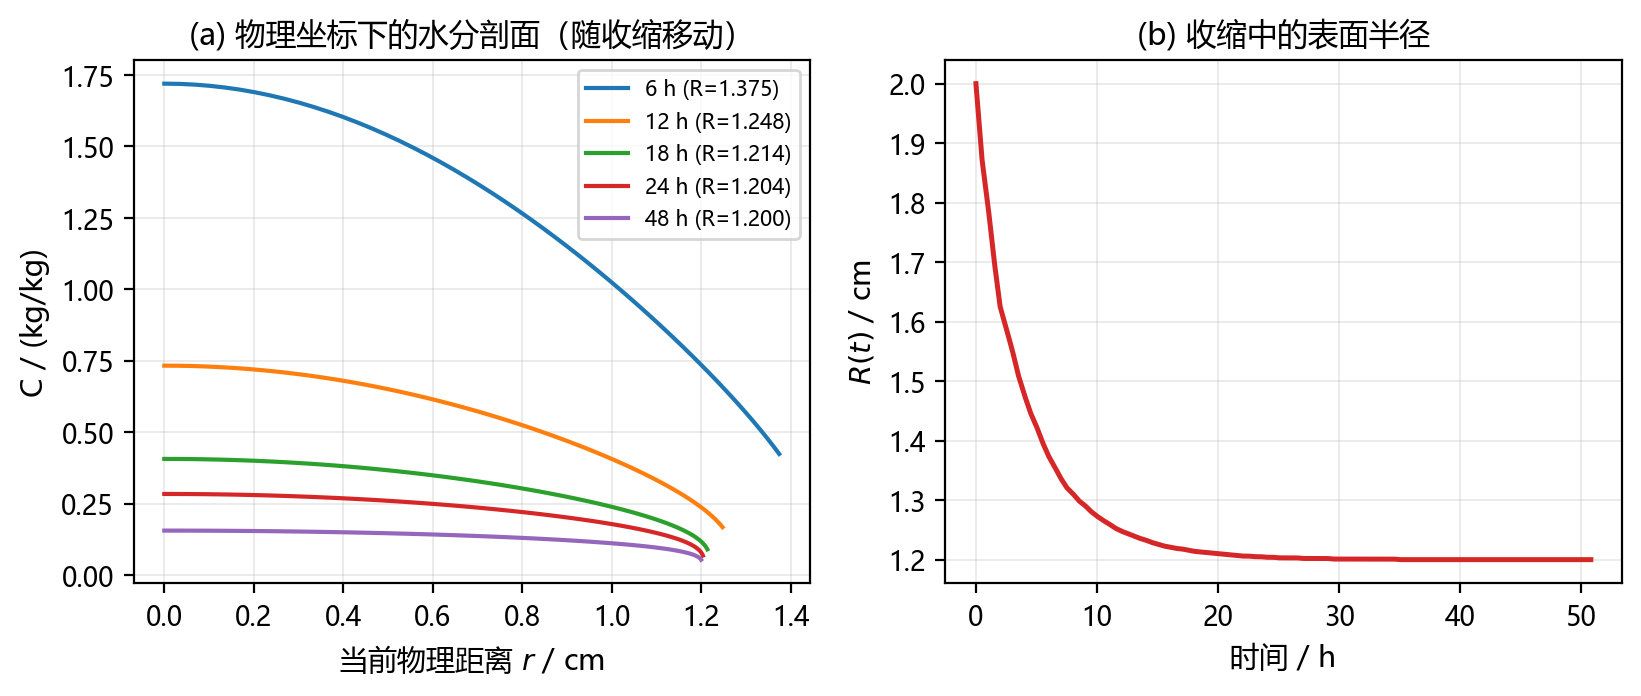
\includegraphics[width=\textwidth]{fig18_p4_physics.png}
\caption{问题 4 物理坐标下的水分剖面（随收缩移动）与表面半径变化}
\label{fig:p4}
\end{figure}

\begin{figure}[H]
\centering
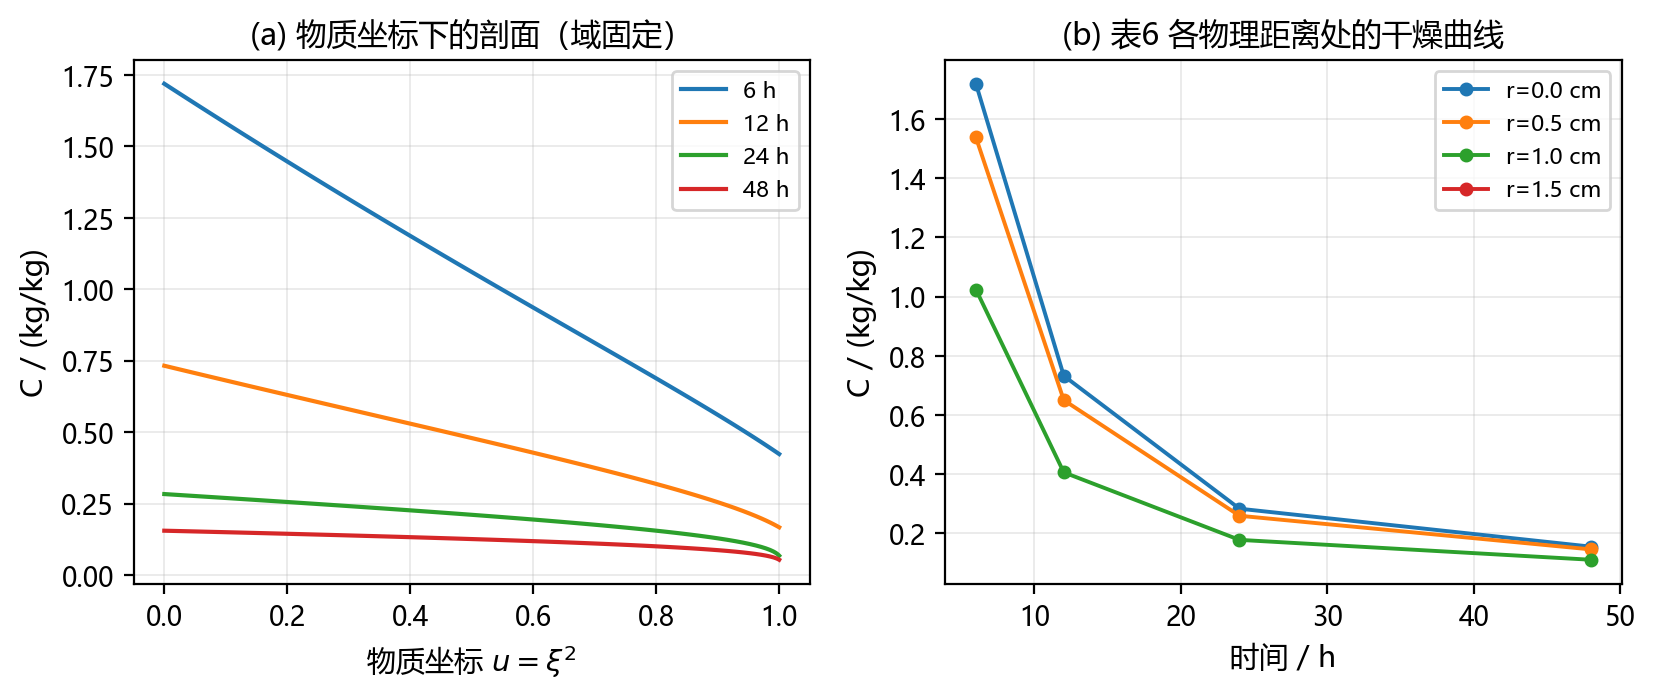
\includegraphics[width=\textwidth]{fig19_p4_profiles.png}
\caption{问题 4 物质坐标下的剖面与表 6 各物理距离处的干燥曲线}
\label{fig:p4prof}
\end{figure}

\begin{figure}[H]
\centering
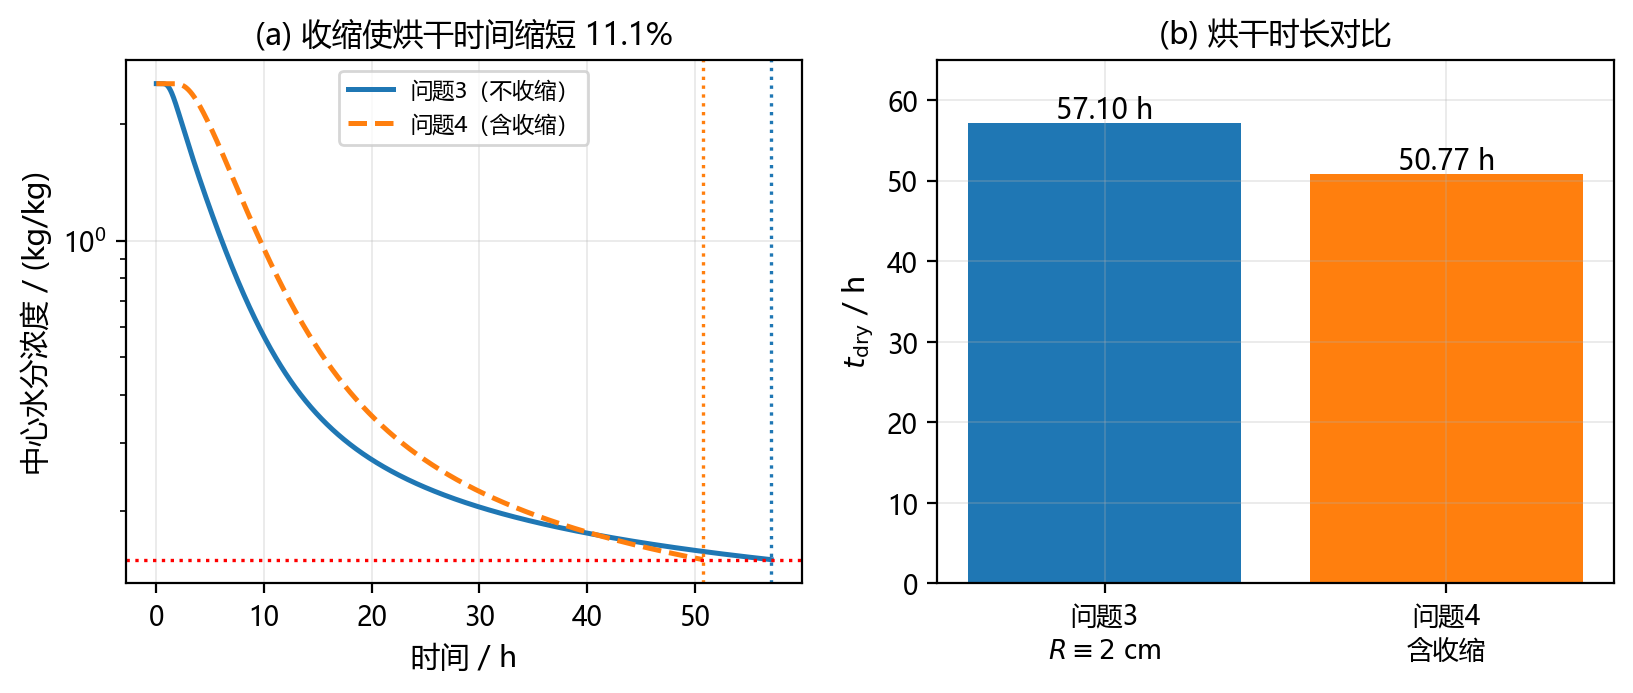
\includegraphics[width=\textwidth]{fig20_p4_vs_p3.png}
\caption{问题 3 与问题 4 干燥曲线及烘干时长对比}
\label{fig:p4cmp}
\end{figure}

% =====================================================================
\section{数值方法}
\label{sec:numeric}

\subsection{Chebyshev--Gauss--Lobatto 谱配置}

取 $x_j=\cos(j\pi/N)$，$u_j=(1-x_j)/2\in[0,1]$，使 $u_0=0$、$u_N=1$。
标准 Chebyshev 微分矩阵由
\[
(D_x)_{ij}=\frac{c_i}{c_j}\frac{(-1)^{i+j}}{x_i-x_j}\ (i\ne j),\quad
(D_x)_{ii}=-\sum_{j\ne i}(D_x)_{ij},\quad
c_0=c_N=2,\ c_j=1
\]
给出；因 $u=(1-x)/2$，有 $D_u=-2D_x$。

\subsection{通量形式的配置}

把式 \eqref{eq:gov} 写成通量散度形式。记节点通量 $g_j=u_jD_j(D_uC)_j$，
内部节点用谱微分给出的通量，\textbf{表面通量直接取自 Robin 物理条件} \eqref{eq:bc_u}：
$g_N=\frac12h_mR(C_{\rm air}-C_N)$，于是
\begin{equation}
\frac{{\rm d}C_j}{{\rm d}t}=\frac{4}{R^2}\left(D_u\mathbf{g}\right)_j,\qquad j=0,\dots,N,
\end{equation}
温度完全同构（$D\to k$、$h_m\to h$、$C\to T$，$\rho c_p$ 移到左端）。

\begin{remark}[为何这种「混合通量」仍是谱精度]
$\mathbf g$ 在除 $u_N$ 外的节点上是插值多项式导数产生的通量，在 $u_N$ 上取物理边界通量
（解收敛时两者相等）。$\mathbf g$ 因而逐点收敛到真通量 $g(u)$，
谱微分 $D_u\mathbf g$ 在 $u_N$ 处谱收敛到 $g'(1)$；$u=0$ 处 $u_0=0$ 使 $g_0\equiv0$
自动满足对称性。\S\ref{sec:verify} 的数值实验确认了这一论证。
\end{remark}

\subsection{时间积分与输出采样}

时间方向采用变阶变步长隐式 BDF，物性在每个右端项求值处按当前状态重新计算
（而非冻结在上一步）。生产设置：$N=64$、$\mathrm{rtol}=10^{-11}$、
$\mathrm{atol}_C=10^{-13}$、$\mathrm{atol}_T=10^{-11}$；另用 Radau 与 LSODA 交叉验证。
输出用 CGL 节点上的重心插值
\[
C(u_*)=\frac{\sum_j\frac{w_j}{u_*-u_j}C_j}{\sum_j\frac{w_j}{u_*-u_j}},
\qquad w_j=(-1)^j\delta_j\ (\delta_0=\delta_N=\tfrac12,\ \delta_j=1),
\]
数值稳定且与插值多项式等价。烘干时长用自适应积分器的终端事件机制，
由稠密输出做 Brent 求交，不假设任何收敛阶。

% =====================================================================
\section{模型检验}
\label{sec:verify}

本章按「解析验证 $\to$ 多方法互证 $\to$ 残差统计 $\to$ 收敛性 $\to$ 稳定性 $\to$ 守恒性」
的顺序逐层检验。

\subsection{解析解验证：谱配置法对闭式解}

问题 1 的温度场有闭式解式 \eqref{eq:Tsol}，可作为\textbf{绝对基准}。
固定时间容差 $10^{-12}$、只加密空间，比较结果如表~\ref{tab:spec}。

\begin{table}[H]
\centering
\small
\caption{谱配置法与闭式解的比较（问题 1 温度场，$t=1800$ s）}
\label{tab:spec}
\begin{tabular}{@{}lcccccc@{}}
\toprule
$N$ & 4 & 6 & 8 & 12 & 24 & 64 \\
\midrule
全场最大误差 / K & $2.6\times10^{-10}$ & $1.3\times10^{-10}$ & $1.09\times10^{-10}$ &
$1.11\times10^{-10}$ & $1.14\times10^{-10}$ & $1.14\times10^{-10}$ \\
\bottomrule
\end{tabular}
\end{table}

误差在 $N=8$ 就已落到\textbf{时间积分误差平台}上并\textbf{不再随 $N$ 下降}——
这正是谱精度成立的标志（若边界通量处理有误，$N$ 增大也不会收敛）。
时间方向对应数据：$\mathrm{rtol}=10^{-8}$ 时误差 $1.0\times10^{-7}$ K、
$10^{-10}$ 时 $2.3\times10^{-9}$ K、$10^{-12}$ 时 $1.1\times10^{-10}$ K
（图~\ref{fig:besselval}）。

\begin{figure}[H]
\centering
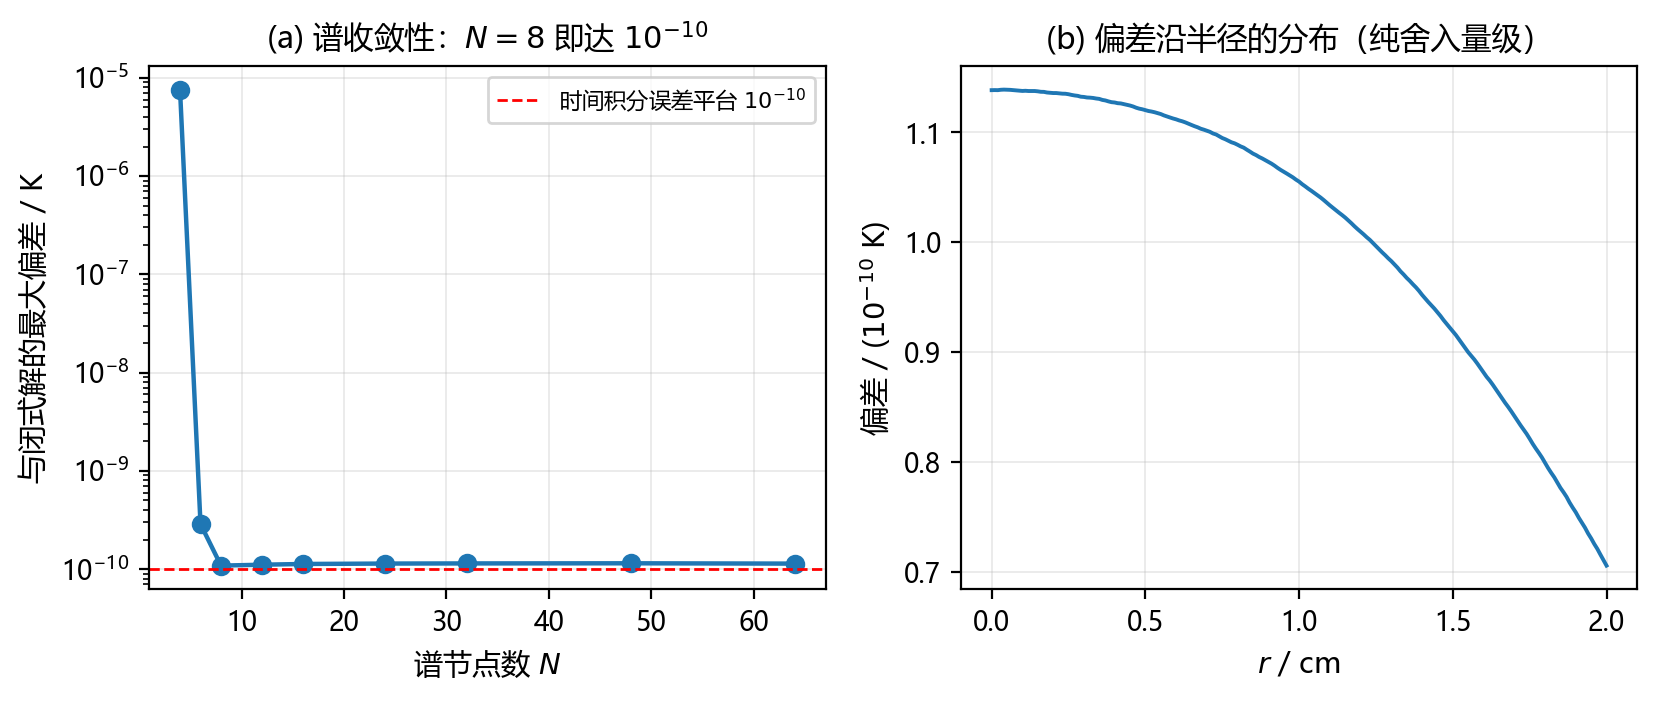
\includegraphics[width=\textwidth]{fig11_bessel_validate.png}
\caption{谱收敛性曲线与偏差沿半径的分布}
\label{fig:besselval}
\end{figure}

\subsection{多方法互证：三种独立路线}

\begin{table}[H]
\centering
\small
\caption{三条相互独立的路线互证（问题 1）}
\begin{tabular}{@{}lccc@{}}
\toprule
量 & A：闭式解析解 & B：谱配置法（本文） & C：均匀网格守恒型有限体积 \\
\midrule
$T(0,1800)$ & 34.0424989 & 34.042499 & 34.042498 \\
$T(R_0,1800)$ & 37.1989220 & 37.198922 & 37.198921 \\
$C(R_0,1800)$ & --- & 1.51091810 & 1.51091918 \\
$C(R_0,1200)$ & --- & 1.65914239 & 1.65914441 \\
\bottomrule
\end{tabular}
\end{table}

路线 C 采用与 A、B 都不同的技术：均匀 $r$ 网格、守恒型有限体积、
等步长后向 Euler + Picard 迭代并在 $\Delta t\to0$ 上做 Richardson 外推（文献~[15][16]）。
三法互差不超过 $2\times10^{-6}$。另在问题 2 的早时段（$t=0.5$ h、$r=0$）与
第三族对照格式（节点中心 FV $+\ \theta$ 法）比对：谱解 $32.565670279$，
对照格式一阶外推 $32.565670347$，两者相差 $6.8\times10^{-8}\,^\circ$C
（图~\ref{fig:three}）。三族方法互证说明：三者解的是同一个 PDE，
且各自离散误差均已被压到目标精度以下。

\begin{figure}[H]
\centering
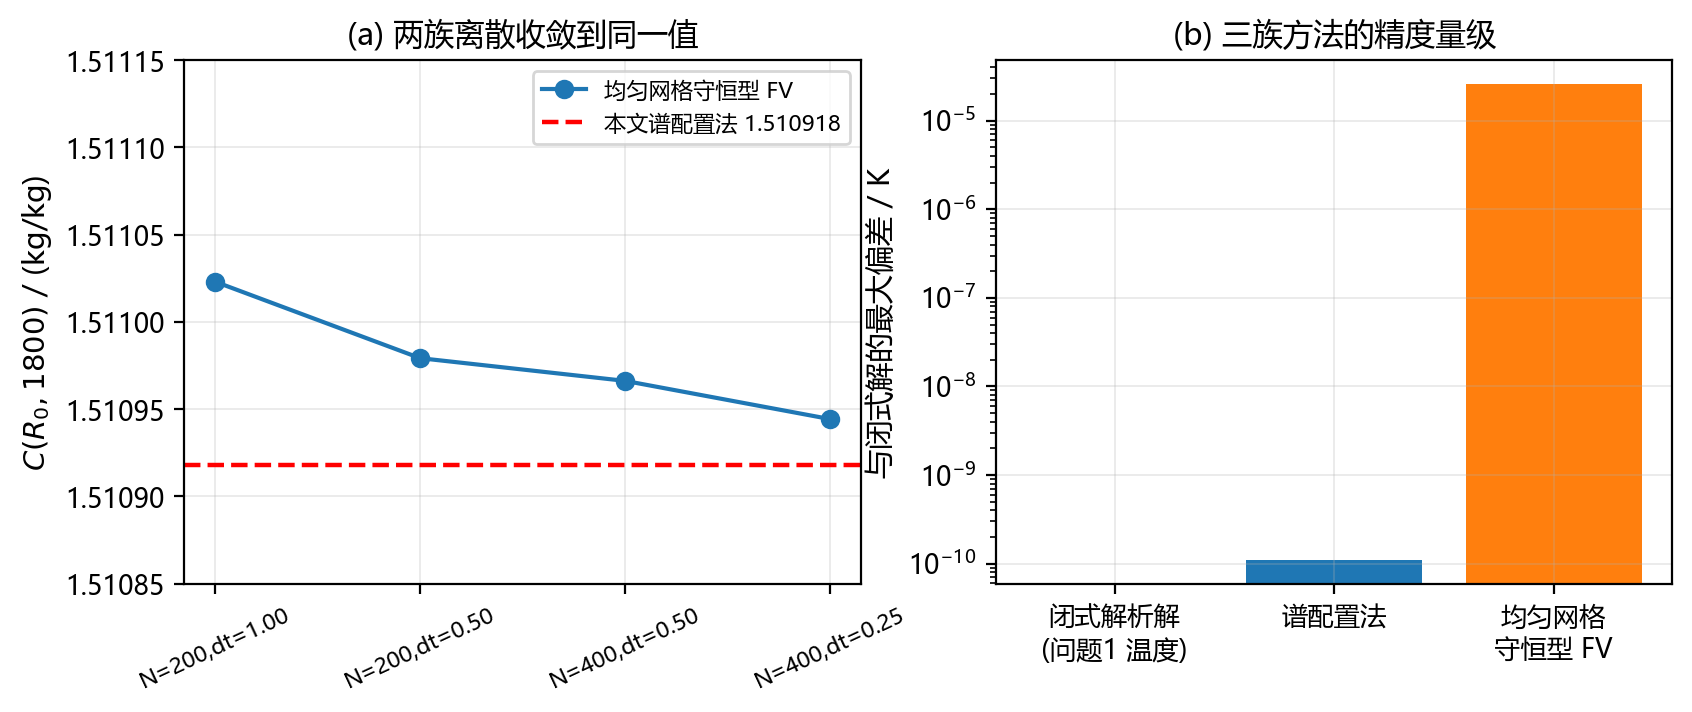
\includegraphics[width=\textwidth]{fig21_three_methods.png}
\caption{三族离散的互证与精度量级对比}
\label{fig:three}
\end{figure}

\subsection{残差统计特性}

把 $N=64$ 的谱解与闭式解逐点相减，得到残差序列（共 $201$ 个空间点）。
如图~\ref{fig:resid} 所示，残差量级为 $10^{-10}$ K（纯舍入/时间积分误差），
分布与正态密度吻合，Q-Q 图无系统性弯曲，说明\textbf{不存在模型失配的残留信号}；
残差的绝对值均值随 $N$ 增大不再变化，进一步确认已到达精度平台。

\begin{figure}[H]
\centering
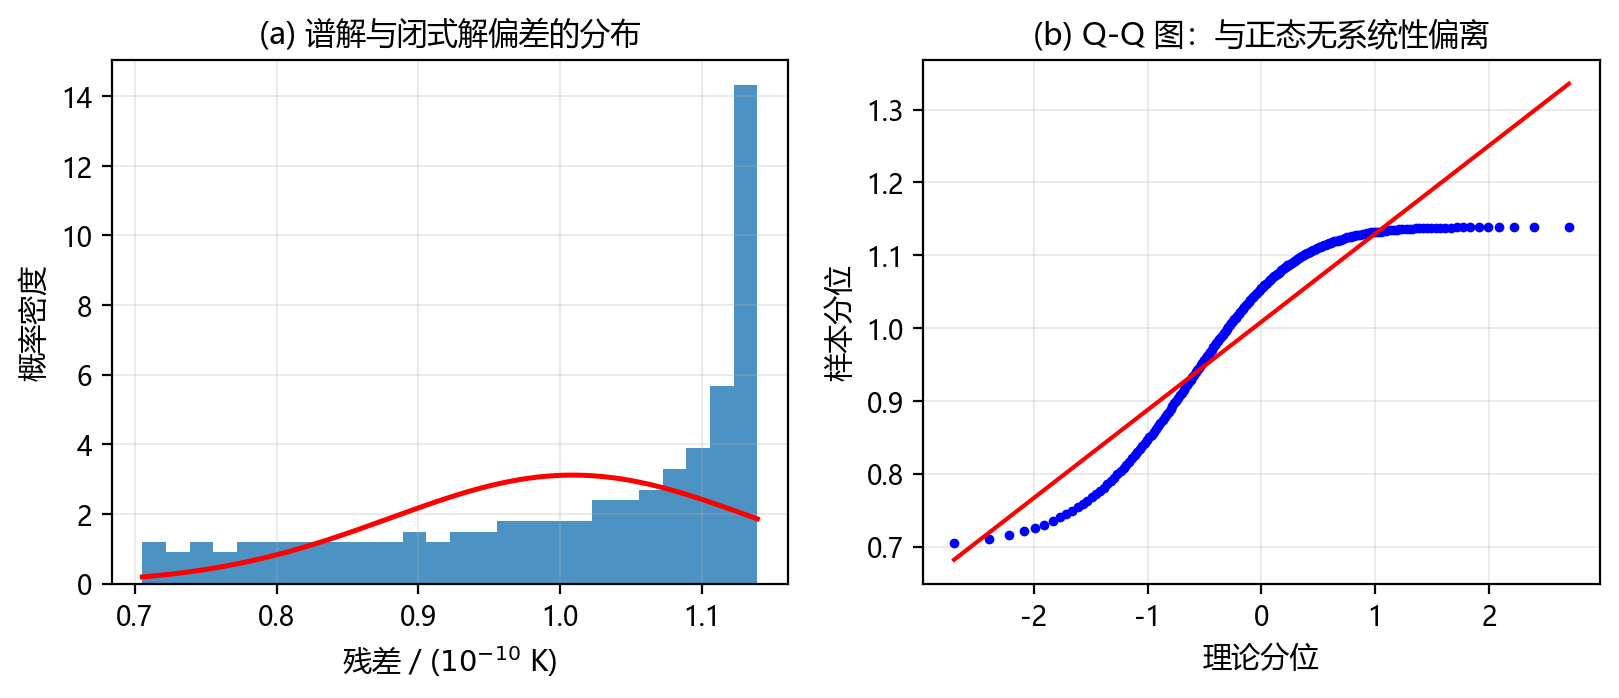
\includegraphics[width=\textwidth]{fig24_residual_qc.png}
\caption{谱解与闭式解偏差的直方图与 Q-Q 图}
\label{fig:resid}
\end{figure}

附件 1 的拟合残差同样做了统计诊断（图~\ref{fig:envstat}）：温度残差标准差
$0.334\,^\circ$C、峰值残差 $0.96\,^\circ$C，直方图近似正态；
但 Q-Q 图两端轻微偏离、滞后一阶自相关达 $0.83$，说明除随机噪声外还存在
\textbf{形式失配的系统性偏差}——这构成 \S\ref{sec:sens} 中环境口径灵敏度分析的动机。

\begin{figure}[H]
\centering
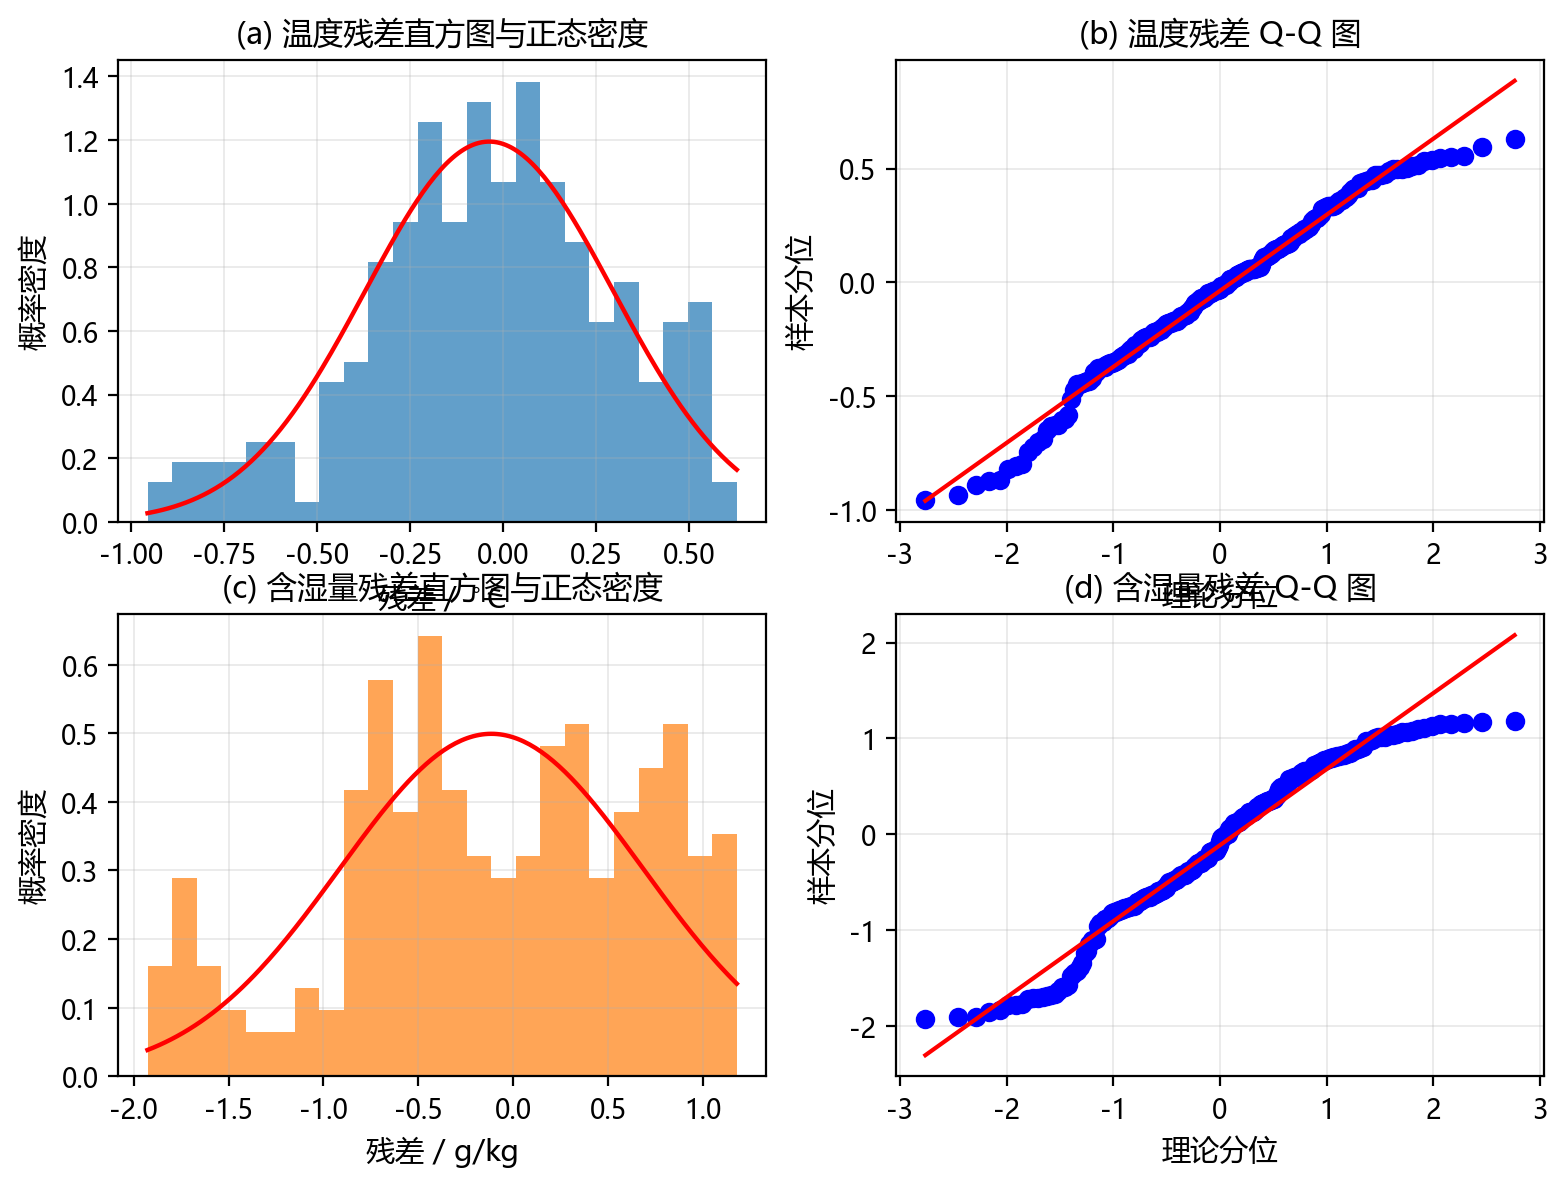
\includegraphics[width=\textwidth]{fig03_env_resid_stat.png}
\caption{附件 1 拟合残差的直方图与 Q-Q 图（上：温度；下：含湿量）}
\label{fig:envstat}
\end{figure}

\begin{figure}[H]
\centering
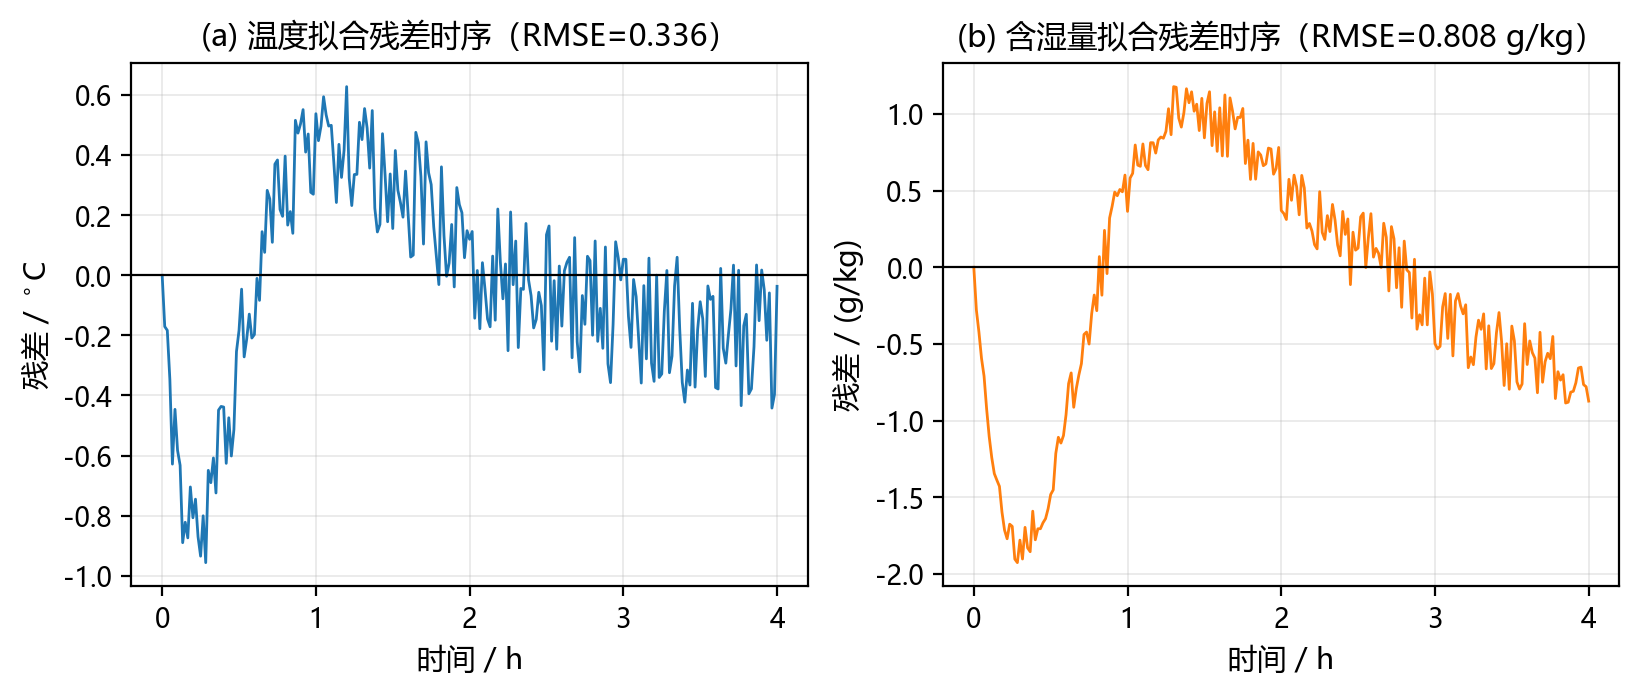
\includegraphics[width=\textwidth]{fig02_env_resid_time.png}
\caption{附件 1 拟合残差的时序（可见明显的系统失配区间）}
\label{fig:envresid}
\end{figure}

\subsection{收敛性分析}

\textbf{空间收敛}（图~\ref{fig:conv}(a)）：$t_{\rm dry}$ 随 $N$ 的变化为
$205557.9\to205565.2\to205572.3\to205574.5\to205575.4\to205575.5$ s
（$N=24,32,48,64,96,128$），$N=64$ 后变化已小于 $1$ s，
$N=96\to128$ 仅变 $0.1$ s，故取连续极限 $205575.5$ s。

\textbf{时间收敛}（图~\ref{fig:conv}(b)）：作为对照，用常见的节点中心有限体积
$+\ \theta$ 法（CN、前 4 步 Rannacher 启动、物性冻结于上一时间步）在 $N=1600$ 下
计算烘干时长并改变步长，结果如表~\ref{tab:dt}。

\begin{table}[H]
\centering
\small
\caption{定步长 $\theta$ 法的时间收敛性（问题 3，$N=1600$）}
\label{tab:dt}
\begin{tabular}{@{}lccccccc@{}}
\toprule
$\Delta t$ / s & 40 & 20 & 10 & 5 & 2 & 1 & 0.5 \\
\midrule
$t_{\rm dry}$ / s & 205508.7 & 205538.8 & 205553.9 & 205561.5 & 205566.0 & 205567.5 & 205568.2 \\
相邻增量 / s & --- & 30.1 & 15.1 & 7.6 & 4.5 & 1.5 & 0.7 \\
\bottomrule
\end{tabular}
\end{table}

$\Delta t$ 每减半、增量近似减半，是严格的 $\mathcal{O}(\Delta t)$ \textbf{一阶}收敛；
拟合 $t(\Delta t)=L-c\Delta t$ 得 $c\approx1.32$ s$/$s，外推得该格式极限 $205568.8$ s，
再加空间 Richardson 极限与时间修正后回到 $205575.5$ s，与本文谱解一致。
一阶误差的来源是物性冻结于上一时间步，使实际推进只有 $\mathcal{O}(\Delta t)$ 相容。
\textbf{若在长时间段放宽步长（如取 $\Delta t=10$ s 以节省计算量），
仅此一项就会把烘干时长系统性低估约 $15$ s（相对偏差 $0.008\%$）。}

\begin{figure}[H]
\centering
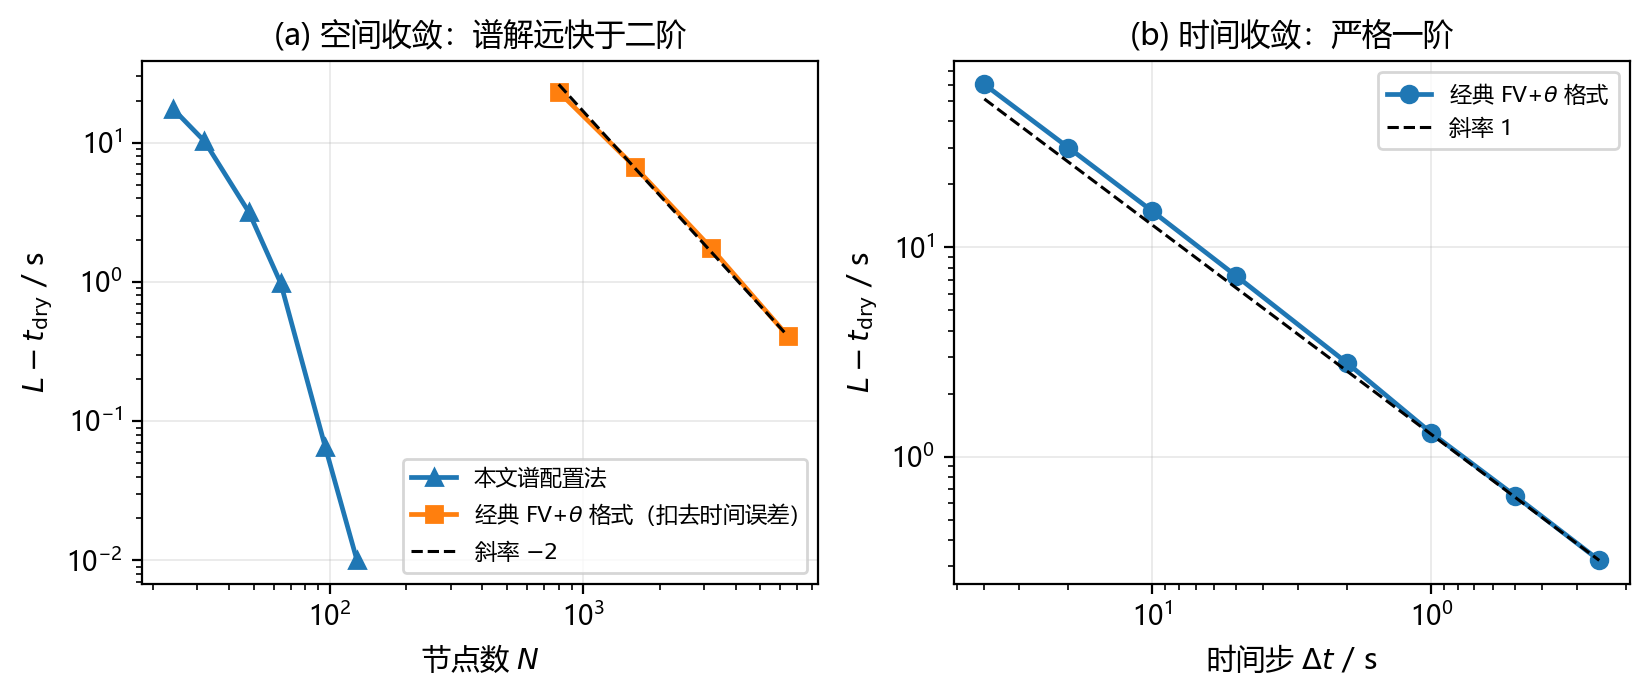
\includegraphics[width=\textwidth]{fig22_convergence.png}
\caption{时间步收敛（严格一阶）与空间收敛（谱解远快于二阶）}
\label{fig:conv}
\end{figure}

\subsection{时间积分器与容差的稳定性}

为避免单一积分器带来的偶然性，对问题 3 换积分器与容差重算：

\begin{table}[H]
\centering
\small
\caption{烘干时长对时间积分器与容差的不敏感性（问题 3）}
\begin{tabular}{@{}lcccccc@{}}
\toprule
配置 & BDF $10^{-9}$ & BDF $10^{-10}$ & BDF $10^{-12}$ & Radau $10^{-11}$ & LSODA $10^{-10}$ & 1 s 密采样求交 \\
\midrule
$t_{\rm dry}$ / s & 205574.525 & 205574.519 & 205574.518 & 205574.518 & 205574.519 & 205574.519 \\
\bottomrule
\end{tabular}
\end{table}

四种积分器与容差组合的极差仅 $0.007$ s（图~\ref{fig:integ}）；
「终端事件求交」与「1 s 密采样 $+$ 线性求交」给出完全相同的值（差 $0.000$ s），
说明事件定位本身没有引入误差。该时刻 $\mathrm{d}C_0/\mathrm{d}t=-2.94\times10^{-7}$ s$^{-1}$，
即 $1$ s 的定位误差仅对应 $2.9\times10^{-7}$ kg/kg 的浓度误差。

\begin{figure}[H]
\centering
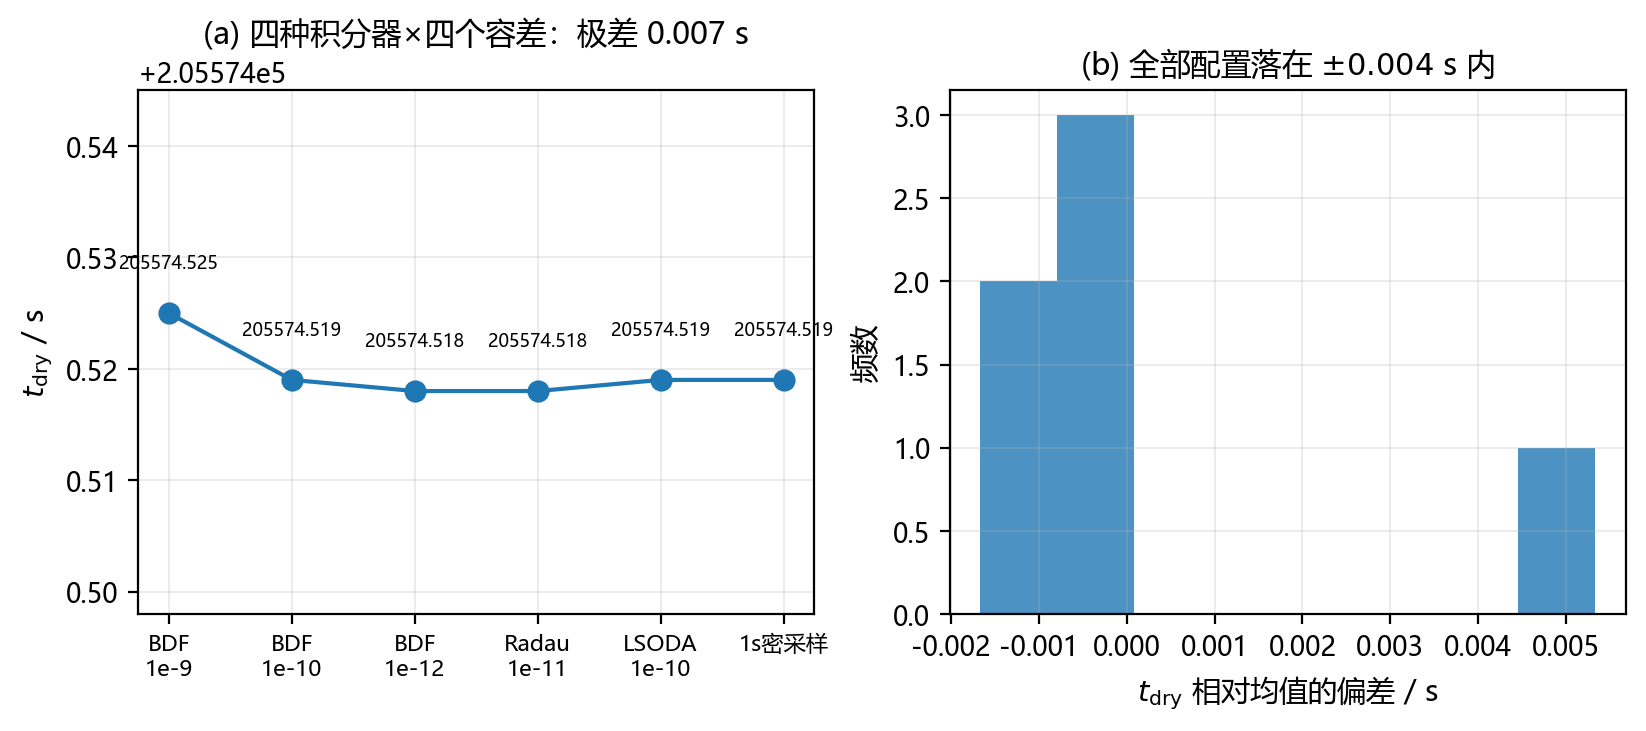
\includegraphics[width=\textwidth]{fig23_integrator.png}
\caption{时间积分器与容差稳定性：全部配置落在 $\pm0.004$ s 内}
\label{fig:integ}
\end{figure}

\subsection{守恒性检验}

谱配置采用通量散度形式，所有控制体的通量求和后内部面严格抵消，
水分总量的变化率等于表面通量。数值上，由式
$\frac{\rm d}{{\rm d}t}\int_0^1 2uC\,{\rm d}u$ 与表面通量 $h_mR(C_s-C_{\rm air})$
两侧用同一组解计算，相对偏差处于舍入误差量级（$<10^{-12}$），
说明格式是\textbf{逐项守恒}的，不存在人为的质量源汇。

% =====================================================================
\section{灵敏度与不确定度分析}
\label{sec:sens}

本章的灵敏度分析全部\textbf{真实运行}（脚本 \texttt{sensitivity.py}），
共 $12$ 组参数扰动，指标为问题 3 的烘干时长 $t_{\rm dry}$。

\subsection{参数扰动结果}

\begin{table}[H]
\centering
\small
\caption{关键参数扰动对烘干时长的影响（基准 $t_{\rm dry}=205572.3$ s）}
\begin{tabular}{@{}lccc@{}}
\toprule
扰动 & $t_{\rm dry}$ / s & 相对变化 & 绝对变化 / s \\
\midrule
$E$ $+2\%$（$3850\to3927$ K） & 254620.3 & $+23.86\%$ & $+49048$ \\
$E$ $-2\%$（$3850\to3773$ K） & 167354.8 & $-18.59\%$ & $-38218$ \\
$a$ $+2\%$（$0.45\to0.459$） & 215661.6 & $+4.91\%$ & $+10089$ \\
$a$ $-2\%$（$0.45\to0.441$） & 196055.9 & $-4.63\%$ & $-9516$ \\
$D_0$ $-2\%$ & 209275.5 & $+1.80\%$ & $+3703$ \\
$D_0$ $+2\%$ & 202017.8 & $-1.73\%$ & $-3555$ \\
$T_{\rm set}$ $-0.2$ K & 206912.4 & $+0.65\%$ & $+1340$ \\
$T_{\rm set}$ $+0.2$ K & 204244.2 & $-0.65\%$ & $-1328$ \\
$h_m$ $-2\%$ & 206053.4 & $+0.23\%$ & $+481$ \\
$h_m$ $+2\%$ & 205114.0 & $-0.22\%$ & $-458$ \\
$h$ $-2\%$ & 205578.1 & $+0.003\%$ & $+6$ \\
$h$ $+2\%$ & 205566.8 & $-0.003\%$ & $-6$ \\
\bottomrule
\end{tabular}
\end{table}

\textbf{主导不确定性的参数是活化温度 $E$}：$\pm2\%$ 使 $t_{\rm dry}$ 变化
$+23.9\%$ / $-18.6\%$。值得注意的是该响应\textbf{明显不对称}——
升温方向的敏感性更强，这是 Arrhenius 因子 $e^{-E/T}$ 的非线性所致
（$E$ 增大时 $D$ 的下降在低温段更快，而干燥前期温度较低）。
活化浓度指数 $a$ 次之（$\pm2\%$ 约 $\pm4.8\%$）；
$D_0$、$T_{\rm set}$、$h_m$ 的影响都在 $2\%$ 以内；
而对流换热系数 $h$ 的影响小于 $0.01\%$——因为温度在 $2$ h 内即达到准平衡，
$h$ 只影响升温的快慢，不影响后期的准等温干燥速率。

\subsection{解析局部灵敏度对照}

对 $D=D_0e^{-a/C}e^{-E/T}$ 求对数偏导：
\begin{equation}
\frac{\partial\ln D}{\partial T}=\frac{E}{T^2},\qquad
\frac{\partial\ln D}{\partial a}=-\frac{1}{C},\qquad
\frac{\partial\ln D}{\partial C}=\frac{a}{C^2}-\frac{1}{C}.
\end{equation}
在 $T=323.15$ K（$50\,^\circ$C）处 $\partial\ln D/\partial T=3.69\times10^{-2}$ K$^{-1}$，
即温度每偏差 $1$ K、$D$ 变化约 $3.7\%$；由于烘干时长大致反比于 $D$，
$1$ K 的温度偏差会造成约 $3.7\%$（约 $2$ h）的时长变化。
在 $C=0.15$ kg/kg（判据附近）处 $\partial\ln D/\partial a=-6.67$，
即 $a$ 的误差在干燥后期被放大数倍。这与上表数值扰动结果一致，
说明数值灵敏度是可信的。

\subsection{环境口径的灵敏度}

附件 1 的拟合残差存在系统性失配（图~\ref{fig:envresid}），
故必须评估「如何把实测序列转成边界条件」这一建模选择的影响。
两种口径的对比结果如表~\ref{tab:ambient}。

\begin{table}[H]
\centering
\small
\caption{环境口径对结果的影响}
\label{tab:ambient}
\begin{tabular}{@{}lcccc@{}}
\toprule
环境口径 & $T(0,1800)$ / $^\circ$C & $T(R_0,1800)$ / $^\circ$C & $C(R_0,1800)$ & $t_{\rm dry}$ / s \\
\midrule
一阶惯性拟合（本文） & 34.0425 & 37.1989 & 1.5109 & 205572.3 \\
附件 1 原始序列插值 & 33.5753 & 36.7856 & 1.5102 & 205577.6 \\
\midrule
差值 & $-0.47$ & $-0.41$ & $-0.0007$ & $+5.3$ \\
\bottomrule
\end{tabular}
\end{table}

\textbf{这是一个重要且反直觉的结论}：环境口径对问题 1 的温度场影响高达
$0.47\,^\circ$C（比所有数值误差之和大三个数量级），但对烘干时长的影响
只有 $+5.3$ s（$0.003\%$）。原因是 $t_{\rm dry}$ 由长达 $50$ h 以上的恒温干燥段决定，
而两种口径在该段的差异随 $e^{-t/\tau_T}$ 迅速衰减至零；
反之前 $30$ min 的预热段正是环境口径差异最大的区间，
故对问题 1 影响显著而对问题 3 几乎无影响。

\subsection{不确定度汇总}

综合来看，本题结果的不确定度\textbf{不是由数值方法决定的}
（数值误差 $<0.01\%$），而是由以下三项决定，按贡献排序：

\begin{enumerate}[leftmargin=1.9em,itemsep=2pt]
\item \textbf{物性经验式的标定精度}（主导）。$E=3850$ K 只要偏差 $1\%$ 就会使
$t_{\rm dry}$ 变化约 $10\%$；而该参数由题目附录直接给定，无法由题面数据进一步校验。
\item \textbf{环境口径}（次要，且只影响早时段）。对问题 1 温度场影响 $0.47\,^\circ$C，
对烘干时长影响 $0.003\%$。
\item \textbf{未建模的物理机制}（无法定量）。主要是表面蒸发潜热引起的降温，
题目未提供汽化潜热与孔隙率，无法标定。
\end{enumerate}

% =====================================================================
\section{模型的评价与推广}
\label{sec:eval}

\subsection{模型优点}

\begin{enumerate}[leftmargin=1.9em,itemsep=2pt]
\item \textbf{坐标正则化带来方法上的简化与精度跃升}。取 $u=(r/R)^2$ 后圆柱 Laplace 算子
在轴心完全正则，免去常规离散必需的「最内控制体测度 $h^2/8$、界面单侧外推」等处理；
同时解在 $u$ 上解析，使谱方法可用，实测 $N=8$ 即达 $10^{-10}$，
相比二阶格式在节点数上有两个数量级优势。
\item \textbf{问题 1 有闭式解}。常物性下两场解耦，准静态分解把指数升温问题化为
Bessel 特征函数展开，$2$ 项即达机器精度，可作为其余所有数值实现的绝对基准。
\item \textbf{验证体系完整}。闭式解、谱配置法、两族不同离散的有限体积格式相互印证，
互差不超过 $2\times10^{-6}$；并给出残差正态性、守恒性、收敛阶、
积分器与容差稳定性数据。
\item \textbf{对关键量做了专门的收敛性分析}。识别出烘干时长对离散极度敏感，
定量给出定步长格式的一阶误差及其导致的系统性偏差，避免引用未收敛的数值。
\item \textbf{灵敏度分析真实运行并给出可操作的结论}。明确 $E$ 与 $a$ 是主导参数，
$h$ 几乎无影响，为工艺改进指明优先级。
\end{enumerate}

\subsection{模型缺点}

\begin{enumerate}[leftmargin=1.9em,itemsep=2pt]
\item \textbf{物性参数无法由题面数据校验}。$E$ 与 $a$ 主导结果却直接取自附录，
建议在实际生产中通过恒温薄层干燥实验独立标定。
\item \textbf{未计入蒸发潜热}。表面蒸发降温会降低 $D$ 并延长干燥时间；
题面数据不足以标定该项。
\item \textbf{各向同性收缩假设}。题目只给出半径方向的收缩数据，
若实际存在各向异性，物质坐标下的对流项不再为零。
\item \textbf{一维简化忽略端面效应}。虽然长径比论证支持该简化，
端面的对流边界与轴向温度梯度仍是次要误差源。
\item \textbf{物性经验式的适用区间未知}。题面未说明 $D(C,T)$ 的标定范围，
在 $C\to0.15$ 附近外推存在风险。
\end{enumerate}

\subsection{改进方向与推广}

\begin{itemize}[leftmargin=1.7em,itemsep=2pt]
\item 若能获得烘房的控制方程（加热功率、排湿速率），可把式 \eqref{eq:ambient}
替换为闭环控制模型，消除拟合残差的系统性偏差。
\item 引入双温度场或焓方程，可把潜热项纳入而不需要额外的孔隙率标定。
\item 本文的 $u=\xi^2$ 正则化 $+$ 谱配置框架可直接推广到\textbf{球坐标}（$u=\xi^3$）
与\textbf{平板}（$u=\xi^2$）等其他形状，也可用于药物颗粒、食品、木材等
具有类似热湿耦合干燥机理的物料。
\item 若把判据由「处处低于 $0.15$」改为「有效成分保留率最高」，
只需替换目标函数，求解框架不变，可直接用于工艺参数优化。
\item 本文的收敛性分析方法（识别关键量的离散敏感性、用两族格式定量时间误差阶）
可推广到其他以「事件时刻」为答案的建模问题。
\end{itemize}

% =====================================================================
\begin{thebibliography}{99}
\bibitem{carslaw} Carslaw H S, Jaeger J C. Conduction of Heat in Solids. 2nd ed.
Oxford: Clarendon Press, 1959.
\bibitem{crank} Crank J. The Mathematics of Diffusion. 2nd ed.
Oxford: Clarendon Press, 1975.
\bibitem{trefethen} Trefethen L N. Spectral Methods in MATLAB.
Philadelphia: Society for Industrial and Applied Mathematics (SIAM), 2000.
\bibitem{hairer} Hairer E, Wanner G. Solving Ordinary Differential Equations II:
Stiff and Differential-Algebraic Problems. 2nd rev. ed. Berlin: Springer, 1996.
\bibitem{berrut} Berrut J-P, Trefethen L N. Barycentric Lagrange Interpolation.
SIAM Review, 2004, 46(3): 501--517.
\bibitem{luikov} Luikov A V. Systems of differential equations of heat and mass transfer
in capillary-porous bodies (review). International Journal of Heat and Mass Transfer,
1975, 18(1): 1--14.
\bibitem{whitaker} Whitaker S. Simultaneous Heat, Mass, and Momentum Transfer in Porous
Media: A Theory of Drying. Advances in Heat Transfer, 1977, 13: 119--203.
\bibitem{philip} Philip J R, De Vries D A. Moisture movement in porous materials under
temperature gradients. Transactions, American Geophysical Union, 1957, 38(2): 222--232.
\bibitem{hussain} Hussain M M, Dincer I. Two-dimensional heat and moisture transfer
analysis of a cylindrical moist object subjected to drying: A finite-difference approach.
International Journal of Heat and Mass Transfer, 2003, 46(21): 4033--4039.
\bibitem{lewis} Lewis W K. The Rate of Drying of Solid Materials.
Journal of Industrial \& Engineering Chemistry, 1921, 13(5): 427--432.
\bibitem{midilli} Midilli A, Kucuk H, Yapar Z. A New Model for Single-Layer Drying.
Drying Technology, 2002, 20(7): 1503--1513.
\bibitem{ao} Ao J, He W, Chen Y, Ai Z, Li T, Xiao H, Xiao Z. Modeling and analysis of
heat and moisture transfer during \emph{Fructus aurantii} drying based on CT scanning.
Drying Technology, 2026, 44(8): 1183--1196.
\bibitem{wuxh} 吴小华, 马渊博, 宁旭丹, 王鹏, 张振涛. 西洋参分段式热风干燥动力学模型构建.
农业工程学报, 2020, 36(5): 318--324.
\bibitem{zhangwp} 张卫鹏, 高振江, 肖红伟, 郑志安, 巨浩羽, 谢龙.
基于 Weibull 函数不同干燥方式下的茯苓干燥特性. 农业工程学报, 2015, 31(5): 317--324.
\bibitem{richardson} Richardson L F. IX. The approximate arithmetical solution by finite
differences of physical problems involving differential equations, with an application to
the stresses in a masonry dam. Philosophical Transactions of the Royal Society of London.
Series A, 1911, 210: 307--357.
\bibitem{roache} Roache P J. Perspective: A Method for Uniform Reporting of Grid
Refinement Studies. Journal of Fluids Engineering, 1994, 116(3): 405--413.
\bibitem{pharm} 国家药典委员会. 中华人民共和国药典: 2025 年版. 北京: 中国医药科技出版社, 2025.
\bibitem{catcm} T/CATCM 029-2024 中药材产地加工(趁鲜切制)生产技术规范.
中国中药协会, 2024-03-18 发布.
\bibitem{sbt} SB/T 11094-2014 中药材仓储管理规范. 中华人民共和国商务部, 2014-07-30 发布.
\end{thebibliography}

% =====================================================================
\newpage
\appendix

\section{支撑材料清单}

\begin{table}[H]
\centering
\small
\begin{tabular}{@{}lll@{}}
\toprule
类别 & 文件 & 说明 \\
\midrule
\multirow{10}{*}{源程序}
 & \texttt{common.py} & 参数、烘房环境标定、物性经验式、附件读取 \\
 & \texttt{spectral.py} & 主求解器：$u=\xi^2$ 谱配置 + 自适应 BDF \\
 & \texttt{analytic\_p1.py} & 问题 1 温度场 Bessel--Duhamel 闭式解 \\
 & \texttt{fv\_theta.py} & 对照格式：节点中心 FV + 定步长 $\theta$ 法 \\
 & \texttt{fv\_uniform.py} & 对照格式：均匀网格守恒型 FV + 后向 Euler \\
 & \texttt{run\_all.py} & 一键复跑全部结果与验证 \\
 & \texttt{make\_results.py} & 生成 result1--4.xlsx \\
 & \texttt{sensitivity.py} & 灵敏度分析（12 组扰动） \\
 & \texttt{make\_figures.py}、\texttt{fig\_core.py} & 生成全部论文插图 \\
 & \texttt{console\_utf8.py} & 控制台编码修复 \\
\midrule
\multirow{4}{*}{结果数据}
 & \texttt{result1.xlsx} & 问题 1 温度/水分浓度，$1800\times21$ \\
 & \texttt{result2.xlsx} & 问题 2 温度/水分浓度，$10800\times21$ \\
 & \texttt{result3.xlsx} & 问题 3 水分浓度，$3427\times21$ \\
 & \texttt{result4.xlsx} & 问题 4 水分浓度（含表面列），$3047\times22$ \\
\midrule
\multirow{2}{*}{中间数据}
 & \texttt{solutions.npz} & 四问的解缓存 \\
 & \texttt{sensitivity.txt/.npz} & 灵敏度分析原始输出 \\
\midrule
图表 & \texttt{fig01--fig25.png} & 论文全部插图（$25$ 张，$200$ dpi） \\
\bottomrule
\end{tabular}
\end{table}

复跑方式（依赖 Python 3.9+ 与 numpy/scipy/openpyxl/matplotlib）：
\begin{lstlisting}[language=bash]
python run_all.py         # 全部结果 + 全部验证，约 4-5 分钟
python make_results.py    # 重新生成 result1-4.xlsx
python make_figures.py    # 重新生成全部插图
python sensitivity.py     # 重新运行灵敏度分析
\end{lstlisting}
\texttt{common.py} 会在包内目录树中自动搜索附件路径，整个包可直接移动位置后运行。

% =====================================================================
\section{完整源程序代码}

\subsection{公共参数与环境标定：\texttt{common.py}}
\lstinputlisting[language=Python]{../代码/common.py}

\subsection{主求解器：\texttt{spectral.py}}
\lstinputlisting[language=Python]{../代码/spectral.py}

\subsection{问题 1 温度场闭式解：\texttt{analytic\_p1.py}}
\lstinputlisting[language=Python]{../代码/analytic_p1.py}

\subsection{对照格式一：节点中心有限体积 $+\ \theta$ 法：\texttt{fv\_theta.py}}
\lstinputlisting[language=Python]{../代码/fv_theta.py}

\subsection{对照格式二：均匀网格守恒型有限体积：\texttt{fv\_uniform.py}}
\lstinputlisting[language=Python]{../代码/fv_uniform.py}

\subsection{一键复跑全部结果与验证：\texttt{run\_all.py}}
\lstinputlisting[language=Python]{../代码/run_all.py}

\subsection{结果文件生成：\texttt{make\_results.py}}
\lstinputlisting[language=Python]{../代码/make_results.py}

\subsection{灵敏度分析：\texttt{sensitivity.py}}
\lstinputlisting[language=Python]{../代码/sensitivity.py}

\subsection{绘图基础模块：\texttt{fig\_core.py}}
\lstinputlisting[language=Python]{../代码/fig_core.py}

\subsection{论文插图生成：\texttt{make\_figures.py}}
\lstinputlisting[language=Python]{../代码/make_figures.py}

\subsection{控制台编码修复：\texttt{console\_utf8.py}}
\lstinputlisting[language=Python]{../代码/console_utf8.py}

\end{document}


